%%%%%%%%%%%%%%%%%%%%%%%%%%%%%%%%%%%%%%%%%%%%%%%%
\begin{frame}
		\frametitle{}
		\Background[1] 
	    \begin{center}
		{ {\Huge 第四章~~氢原子~~  (6学时)}}
	    \end{center}    
\end{frame}
%%%%%%%%%%%%%%%%%%%%%%%%%%%%%%%%%%%%%%%%%%%%%xs

\section{1.氢原子薛定谔方程分离变量 }

\subsection{相对坐标系}

\begin{frame}
	\frametitle{氢原子薛定谔方程}
	氢原子含一原子核和一核外电子,是二体问题。\\
	{\Bullet}哈密顿量为:
	\begin{equation*}
		H=\left[-\frac{\hbar^2}{2 m_1} \nabla_1 ^2 + V(\vec{r_1},t) \right]  + \left[-\frac{\hbar^2}{2 m_2} \nabla_2 ^2 + V(\vec{r_2},t) \right]  +U(| \vec{r_1}-\vec{r_2} | )
	\end{equation*}
	其中 V为背景势,U为库仑势(相互作用势):
	\begin{equation*}
		U(| \vec{r_1}-\vec{r_2} | )=-\frac{e_s ^2}{| \vec{r_1}-\vec{r_2} |} ~~,~~~ e_s =\frac{Ze}{\sqrt{4\pi\epsilon_0}}
	\end{equation*}
\end{frame}

\begin{frame}
	\frametitle{}
	{\Bullet}薛定谔方程为:
	\begin{equation*}
		i\hbar \frac{\partial }{\partial t} \Psi (\vec{r_1},\vec{r_2},t ) =H (\vec{r_1},\vec{r_2}, t  )  \Psi (\vec{r_1},\vec{r_2},t ) 
	\end{equation*}
	{\Bullet}当背景势V不显含时间t,时空可分离变量。解得的时间函数为:
	\begin{equation*}
		f(t) =e^{-iEt/\hbar}
	\end{equation*}
	空间函数服从定态薛定谔方程:
	\begin{equation*}
		\left[-\frac{\hbar^2}{2 m_1} \nabla_1 ^2 + V_1  -\frac{\hbar^2}{2 m_2} \nabla_2 ^2 + V_2  +U_{1,2} \right] \Psi (\vec{r_1},\vec{r_2}) =E \Psi (\vec{r_1},\vec{r_2}) 
	\end{equation*}
\end{frame}		

\begin{frame}
	\frametitle{}
	对于自由氢原子,背景势V=0,方程简化为:
	\begin{equation*}
		\left[-\frac{\hbar^2}{2 m_1} \nabla_1 ^2  -\frac{\hbar^2}{2 m_2} \nabla_2 ^2 +U(| \vec{r_1}-\vec{r_2} | ) \right] \Psi (\vec{r_1},\vec{r_2}) =E \Psi (\vec{r_1},\vec{r_2}) 
	\end{equation*}
	其中, 
	\begin{equation*}
		U(| \vec{r_1}-\vec{r_2} | )=-\frac{e_s ^2}{| \vec{r_1}-\vec{r_2} |} 
	\end{equation*}
	这是一个6维势,决定着方程求解的难度.
\end{frame}		

\begin{frame}
	\frametitle{相对坐标}
	{\Bullet} 引入相对坐标和质心坐标\\ \vspace{0.6em}
	令:(1)
	$\displaystyle \begin{cases}
		\vec{r} (x,y,z)= \vec{r_1}-\vec{r_2}  , \qquad \text{(相对坐标)} \\ \vspace{0.3em}
		\vec{R} (X,Y,Z)= \dfrac{ m_1\vec{r_1}+ m_2\vec{r_2}  }{ m_1+m_2} , \qquad \text{(质心坐标)} 
	\end{cases}$ \\	
	\hspace{1.6em} (2)
	$\displaystyle \begin{cases}
		m = \dfrac{m_1m_2}{m_1+m_2}, \qquad \text{(折合质量)}\\
		M= m_1+m_2,  \qquad \text{(质心质量)}
	\end{cases}$ \\	\vspace{1em}
	可实现变量分离!
\end{frame}		

\begin{frame}
	有坐标函数:
	$\displaystyle \begin{cases}
		\vec{r_1}= f_1(\vec{r},\vec{R}) \\
		\vec{r_2}= f_2(\vec{r},\vec{R}) 
	\end{cases}$ \\	
	对其求导:
	\begin{equation*}
		\begin{split}
		\dfrac{d}{dx_1}= &\dfrac{\partial}{\partial X}  \dfrac{\partial X}{ \partial x_1} +\dfrac{\partial }{\partial x}  \dfrac{\partial x}{\partial x_1} 
		= \dfrac{m_1}{M}  \dfrac{\partial }{ \partial X} +\dfrac{\partial }{\partial x} \\ \vspace{0.3em}
		\dfrac{d^2}{dx^2 _1}= &\dfrac{m^2 _1}{M^2 }  \dfrac{\partial^2 }{ \partial X^2} + \dfrac{2m _1}{M }  \dfrac{\partial^2 }{ \partial X \partial x}+\dfrac{\partial ^2 }{\partial x^2} \\		
		\nabla ^2 _1= &\dfrac{m^2 _1}{M^2 }  \nabla ^2 _R + \dfrac{2m _1}{M }  (\dfrac{\partial^2 }{ \partial X \partial x} +  \dfrac{\partial^2 }{ \partial Y \partial y} + \dfrac{\partial^2 }{ \partial Z \partial z})    + \nabla ^2 _r  \\
		\nabla ^2 _2= &\dfrac{m^2 _2}{M^2 }  \nabla ^2 _R - \dfrac{2m _2}{M }  (\dfrac{\partial^2 }{ \partial X \partial x} +  \dfrac{\partial^2 }{ \partial Y \partial y} + \dfrac{\partial^2 }{ \partial Z \partial z})    + \nabla ^2 _r
		\end{split}
	\end{equation*}
\end{frame}		

\begin{frame}
	结合在一起,得:	
	\begin{equation*}
		\dfrac{1}{m_1}\nabla ^2 _1	+ \dfrac{1}{m_2}\nabla ^2 _2 = \dfrac{1}{M}\nabla ^2 _R+ \dfrac{1}{m}\nabla ^2 _r
	\end{equation*}	
	代回简化后的方程,得:
	\begin{equation*}
		\left[-\frac{\hbar^2}{2 M} \nabla_R ^2  -\frac{\hbar^2}{2 m} \nabla_r ^2 +U(\vec{r} ) \right] \Psi (\vec{R},\vec{r}) =E \Psi (\vec{R},\vec{r}) 
	\end{equation*}
	相对和质心坐标可分离变量! \\ 
	令: $\Psi (\vec{R},\vec{r}) = \psi (\vec{R}) \Psi (\vec{r})  $, 代入上方程,
\end{frame}		

\begin{frame}
	\frametitle{质心运动方程}
	得方程(1):
	\begin{equation*}
		-\frac{\hbar^2}{2 M} \nabla_R ^2  \psi (\vec{R}) =E_c \psi (\vec{R})  ..... (1)
	\end{equation*}	
	这是质心运动方程,解为自由粒子平面波:
	\begin{equation*}
	\psi (\vec{R},t)=-\frac{1}{(2\pi\hbar)^{3/2}}e^{-\frac{i}{\hbar}(E_c t -\vec{p}\cdot\vec{R})}
	\end{equation*}
\end{frame}		

\begin{frame}
	\frametitle{相对运动方程}
	不失一般性,方程(2)写为:
	\begin{equation*}
		\left[-\frac{\hbar^2}{2 m} \nabla ^2 +U(\vec{r}) \right] \Psi (\vec{r}) =E \Psi (\vec{r})   ..... (2)
	\end{equation*}
	这是相对运动方程,是核与核外电子相对于质心的运动方程.\\
	可以近似地看成是核外电子相对于核的运动方程.
\end{frame}	

\begin{frame}
	其中,
	\begin{equation*}
		U(\vec{r})=U(| \vec{r_1}-\vec{r_2} | )=-\frac{e_s ^2}{| \vec{r_1}-\vec{r_2} |} = -\frac{e_s ^2}{r} ~~,~~~ r =\sqrt{x^2+y^2+z^2}
	\end{equation*}
	 有
	\begin{equation*}
		U(r)=-\frac{e_s ^2}{r}
	\end{equation*}	
	是一个与角量无关的物理量。 \\
	若改用球坐标系描述方程(2), 则经向r可分离变量!\\
	\begin{equation*}
		\left[-\frac{\hbar^2}{2 \mu} \nabla ^2 +U(r) \right] \Psi (\vec{r}) =E \Psi (\vec{r})   ..... (2)
	\end{equation*}
	因此要求普拉斯算子$\nabla ^2$的球坐标系形式
\end{frame}		

\subsection{球坐标拉普拉斯}

\begin{frame}
	\frametitle{球坐标拉普拉斯算子}
	\例[1.已知x,y,z)坐标系下的拉普拉斯算子为] 
	{\begin{equation*}
		\nabla ^{2}  = \dfrac{\partial ^2}{\partial x^2} +\dfrac{\partial^2 }{\partial y^2} +\dfrac{\partial^2  }{\partial z^2}
	\end{equation*}\\
	求 ($r, \theta, \varphi $)坐标系下的拉普拉斯算子 \\ 
	}
	\begin{center}
		   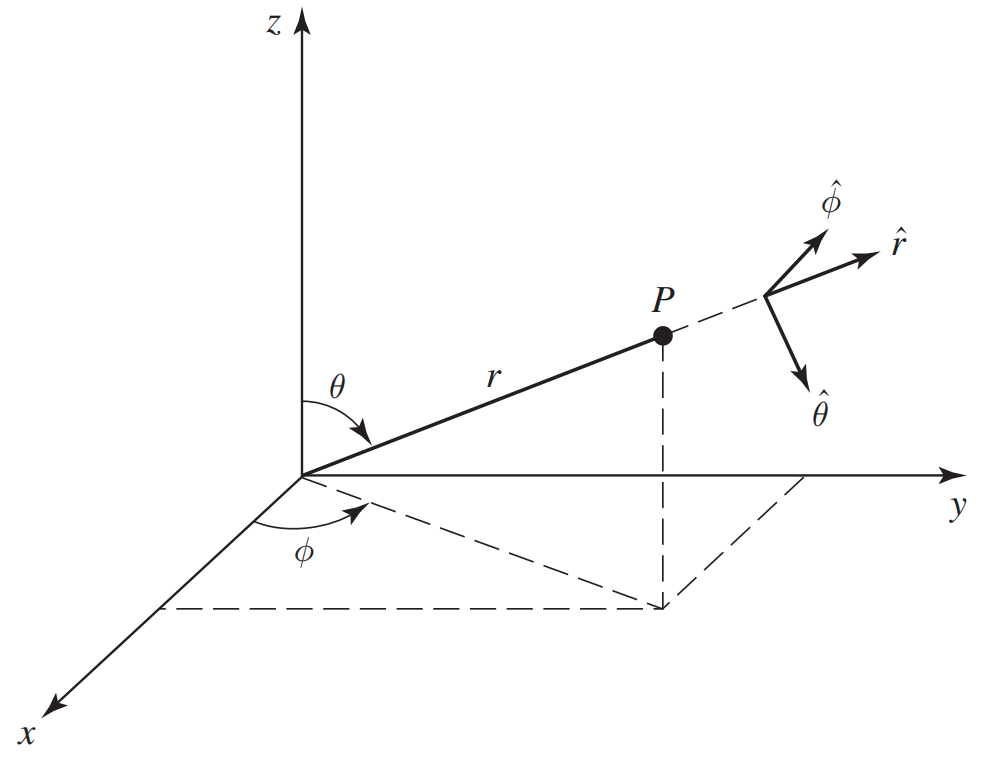
\includegraphics[width=0.48\textwidth]{figs/2022-03-28-22-51-18.png}
	\end{center}
\end{frame}

\begin{frame}
	  \frametitle{}	  
	\alert{解:}  坐标变换关系为:\\
	$\begin{cases}
		x= r\sin \theta \cos \varphi \\
		y= r\sin \theta \sin \varphi \\
		z=r\cos \theta
	\end{cases} $ \\
	对函数$u(x,y,z)$,进行 $r, \theta, \varphi $求导,有:\\ \vspace{0.6em}
	{\small $\begin{cases}
		\dfrac{\partial {u}}{\partial {r}}=\dfrac{\partial {u}}{\partial x} \dfrac{\partial {x}}{\partial {r}}+\dfrac{\partial u}{\partial {y}} \dfrac{\partial {y}}{\partial {r}}+\dfrac{\partial u}{\partial z} \dfrac{\partial z}{\partial {r}} \\ \vspace{0.3em}
		\dfrac{\partial {u}}{\partial \theta}=\dfrac{\partial {u}}{\partial x} \dfrac{\partial{x}}{\partial \theta}+\dfrac{\partial u}{\partial {y}} \dfrac{\partial {y}}{\partial \theta}+\dfrac{\partial{u}}{\partial z} \dfrac{\partial z}{\partial \theta} \\ \vspace{0.3em}
		\dfrac{\partial {u}}{\partial \varphi}=\dfrac{\partial u}{\partial x} \dfrac{\partial{x}}{\partial \varphi}+\dfrac{\partial u}{\partial y} \dfrac{\partial y}{\partial \varphi}+\dfrac{\partial u}{\partial z} \dfrac{\partial z}{\partial \varphi}
	\end{cases} $}\\ \vspace{1em}
\end{frame}	

\begin{frame}
	写成矩阵形式 \\ \vspace{1em}
	{\small $\left[\begin{array}{ccc}
		\dfrac{\partial u}{\partial r} \\ \vspace{0.3em}
		\dfrac{\partial u}{\partial \theta} \\ \vspace{0.3em}
		\dfrac{\partial u}{\partial \varphi}
	\end{array}\right]$
	=
	$\left[\begin{array}{ccc}
		\sin \theta \cos \varphi & \sin \theta \sin \varphi & \cos \theta \\ \vspace{0.3em}
		r \cos \theta \cos \varphi & r \cos \theta \sin \varphi & -r \sin \theta \\ \vspace{0.3em}
		-r \sin \theta \sin \varphi & r \sin \theta \cos \varphi & 0
	\end{array}\right]$
	$\left[\begin{array}{ccc}
		\dfrac{\partial u}{\partial x} \\ \vspace{0.3em}
		\dfrac{\partial u}{\partial y} \\ \vspace{0.3em}
		\dfrac{\partial u}{\partial z}
	\end{array}\right]$
	}\\
	{\small $\left[\begin{array}{ccc}
		\dfrac{\partial u}{\partial r} \\ \vspace{0.3em}
		\dfrac{\partial u}{\partial \theta} \\ \vspace{0.3em}
		\dfrac{\partial u}{\partial \varphi}
	\end{array}\right]$
	=
	$\left[\begin{array}{ccc}
		1 & 0 & 0 \\ \vspace{0.3em}
		0 & r  & 0 \\ \vspace{0.3em}
		0 & 0 & r \sin \theta 
	\end{array}\right]$
	$\left[\begin{array}{ccc}
		\sin \theta \cos \varphi & \sin \theta \sin \varphi & \cos \theta \\ \vspace{0.3em}
		\cos \theta \cos \varphi & \cos \theta \sin \varphi & - \sin \theta \\ \vspace{0.3em}
		-\sin \varphi &  \cos \varphi & 0
	\end{array}\right]$
	$\left[\begin{array}{ccc}
		\dfrac{\partial u}{\partial x} \\ \vspace{0.3em}
		\dfrac{\partial u}{\partial y} \\ \vspace{0.3em}
		\dfrac{\partial u}{\partial z}
	\end{array}\right]$
	}
\end{frame}	

\begin{frame}
	\small {$
		\left[\begin{array}{ccc}
			\dfrac{\partial u}{\partial x} \\
			\dfrac{\partial u}{\partial y} \\
			\dfrac{\partial u}{\partial z}
		\end{array}\right]$
		=
		$\left[\begin{array}{ccc}
			\sin \theta \cos \varphi & \cos \theta \cos \varphi & -\sin \varphi \\
			\sin \theta \sin \varphi &  \cos \theta \sin \varphi &  \cos \varphi \\
			\cos \theta & -\sin \theta & 0
		\end{array}\right]$
		$\left[\begin{array}{ccc}
			\dfrac{\partial u}{\partial r} \\
			\dfrac{1}{r}\dfrac{\partial u}{\partial \theta} \\
			\dfrac{1}{r \sin \theta}\dfrac{\partial u}{\partial \varphi}
		\end{array}\right]
		$}	\\ \vspace{0.3cm}
	\small {$
		\left[\begin{array}{ccc}
			\dfrac{\partial u}{\partial x} \\
			\dfrac{\partial u}{\partial y} \\
			\dfrac{\partial u}{\partial z}
		\end{array}\right]$
		=
		$\left[\begin{array}{ccc}
			{\vec{e}_r}&  {\vec{e}_\theta} & {\vec{e}_\varphi}
		\end{array}\right]$
		$\left[\begin{array}{ccc}
			\dfrac{\partial u}{\partial r} \\
			\dfrac{1}{r}\dfrac{\partial u}{\partial \theta} \\
			\dfrac{1}{r \sin \theta}\dfrac{\partial u}{\partial \varphi}
		\end{array}\right]
		$}	\\ 
\end{frame}	

\begin{frame}
	球坐标系下, 有:
	\begin{equation*}
	\nabla=\vec{e}_{r} \frac{\partial}{\partial r}+\frac{1}{r} \vec{e}_{\theta} \frac{\partial}{\partial \theta}+\frac{1}{r \sin \theta} \vec{e}_{\varphi} \frac{\partial}{\partial \varphi}
	\end{equation*}
	\begin{equation*}
	\begin{split}
		\nabla ^2&=\nabla \cdot \nabla \\
		&=(\vec{e}_{r} \frac{\partial}{\partial r}+\frac{1}{r} \vec{e}_{\theta} \frac{\partial}{\partial \theta}+\frac{1}{r \sin \theta} \vec{e}_{\varphi} \frac{\partial}{\partial \varphi})  \cdot (\vec{e}_{r} \frac{\partial}{\partial r}+\frac{1}{r} \vec{e}_{\theta} \frac{\partial}{\partial \theta}+\frac{1}{r \sin \theta} \vec{e}_{\varphi} \frac{\partial}{\partial \varphi}) \\
		&=\frac{\partial ^2}{\partial r^2} + ( \frac{1}{r} \frac{\partial}{\partial r} + \frac{1}{r^2} \frac{\partial^2} {\partial \theta ^2}  ) + (\frac{1}{r} \frac{\partial}{\partial r}  + \frac{\cos \theta}{r^2 \sin \theta} \frac{\partial} {\partial \theta }  + \frac{1}{r^2 \sin^2 \theta  } \frac{\partial^2}{\partial\varphi ^2} )\\
		&=\frac{1}{r^2} \frac{\partial }{\partial r} (r^2\frac{\partial }{\partial r} )+
		\frac{1}{r^2 \sin \theta  } \frac{\partial }{\partial \theta } (\sin \theta \frac{\partial }{\partial \theta } )
		+\frac{1}{r^2 \sin^2 \theta  } \frac{\partial^2}{\partial\varphi ^2}
	\end{split}
	\end{equation*}

	{\Bullet}~利用球坐标单位矢(1)正交归一性和(2)微分性质完成计算(见讲义 15页)
\end{frame}	

\begin{frame}
	直角坐标~ $(x,y,z) $: 
	\begin{equation*}
		\nabla ^{2}  = \dfrac{\partial ^2}{\partial x^2} +\dfrac{\partial^2 }{\partial y^2} +\dfrac{\partial^2  }{\partial z^2}
	\end{equation*}
	球坐标~ $(r,\theta, \varphi )$ :
	\begin{equation*}
		\nabla ^{2} =\frac{1}{r^2} \frac{\partial }{\partial r} (r^2\frac{\partial }{\partial r} )+
		\frac{1}{r^2 \sin \theta  } \frac{\partial }{\partial \theta } (\sin \theta \frac{\partial }{\partial \theta } )
		+\frac{1}{r^2 \sin^2 \theta  } \frac{\partial^2}{\partial\varphi ^2}
	\end{equation*}	
	令角向部分为:
	\begin{equation*}
		L^2 = - \left[ \frac{1}{ \sin \theta  } \frac{\partial }{\partial \theta } (\sin \theta \frac{\partial }{\partial \theta } )
		+\frac{1}{ \sin^2 \theta  } \frac{\partial^2}{\partial\varphi ^2} \right]
	\end{equation*}	
	有 :
	\begin{equation*}
		\nabla ^{2} =\frac{1}{r^2} \frac{\partial }{\partial r} (r^2\frac{\partial }{\partial r} )-
		\frac{1}{r^2 } L^2 
	\end{equation*}	
	的确它由径向和角向二部分加和构成,因此可实现径向和角向的分离变量!
\end{frame}	

\begin{frame}
	\frametitle{角向与角动量的关系}	
	角向(方)算子:
	\begin{equation*}
		L^2 = - \left[ \frac{1}{ \sin \theta  } \frac{\partial }{\partial \theta } (\sin \theta \frac{\partial }{\partial \theta } )
		+\frac{1}{ \sin^2 \theta  } \frac{\partial^2}{\partial\varphi ^2} \right]
	\end{equation*}	
    角动量(方)算子:
		\begin{equation*}
		L^2 = -\hbar ^2 \left[ \frac{1}{ \sin \theta  } \frac{\partial }{\partial \theta } (\sin \theta \frac{\partial }{\partial \theta } )
		+\frac{1}{ \sin^2 \theta  } \frac{\partial^2}{\partial\varphi ^2} \right]
	\end{equation*}	
	动量的切向分量
	\begin{equation*}
	p_ \perp  ^2 =  \frac{L^2}{r^2}
	\end{equation*}	
	动量的径向分量
	\[ p_r ^2 = -\hbar ^2  \frac{1}{r^2} \frac{\partial }{\partial r} (r^2\frac{\partial }{\partial r} ) \]
\end{frame}		

\begin{frame}
	得动量算子: 
	\[ \hspace{1em}\hat{p}^2 =-\hbar ^2 \nabla ^{2}
		\]
	\[ \hat{p} =-i\hbar \nabla \quad \text{or} \quad i\hbar \nabla\]
	在球坐标系下,
	\[ \hat{p} =-i\hbar  ( \vec{e}_{r} \frac{\partial}{\partial r}+\frac{1}{r} \vec{e}_{\theta} \frac{\partial}{\partial \theta}+\frac{1}{r \sin \theta} \vec{e}_{\varphi} \frac{\partial}{\partial \varphi})
		\]
\end{frame}		

\begin{frame}
	\frametitle{位置算子 }	
	$\begin{cases}
		x= r\sin \theta \cos \varphi \\
		y= r\sin \theta \sin \varphi \\
		z=r\cos \theta
	\end{cases} $\\ 
	~~\\
	矩阵形式: \\ \vspace{0.6em}
	$
	\left[\begin{array}{ccc}
		x \\
		y \\
		z
	\end{array}\right]$
	=
	$\left[\begin{array}{ccc}
		r\sin \theta \cos \varphi  \\
		r\sin \theta \sin \varphi  \\
		r\cos \theta
	\end{array}\right]$	
	=
	$r \vec{e}_r$ \\ \vspace{0.3cm}
	球坐标系下,位置算子:
	\[ \qquad \hat{r}=r \vec{e}_r \]
\end{frame}	

\begin{frame}
	角动量: $ \vec{L}= \vec{r}\times \vec{p} $, \\
	球坐标系下,角动量算子:
	\begin{equation*}
		\hat{L}= \hat{r}\times \hat{p} = -i \hbar r \vec{e}_r \times \nabla  
	\end{equation*}
	\begin{equation*}
		\hat{L}=   -i \hbar   ( \vec{e}_{\varphi} \frac{\partial}{\partial \theta} - \frac{1}{\sin \theta}  \vec{e}_{\theta} \frac{\partial}{\partial \varphi} )
	\end{equation*}
	\begin{equation*}
		\begin{split}
		\hat{L}	^2 &=   - \hbar ^2  ( e_{\varphi} \frac{\partial}{\partial \theta} - \frac{1}{\sin \theta}  e_{\theta} \frac{\partial}{\partial \varphi} )  \cdot   ( e_{\varphi} \frac{\partial}{\partial \theta} - \frac{1}{\sin \theta}  e_{\theta} \frac{\partial}{\partial \varphi} ) \\
		&= - \hbar ^2 (\frac{1}{\sin \theta  } \frac{\partial }{\partial \theta } (\sin \theta \frac{\partial }{\partial \theta } )
		+\frac{1}{\sin^2 \theta  } \frac{\partial^2}{\partial\varphi ^2} ) 	
		\end{split}
	\end{equation*}
	正是前面的假设, 完全自洽!\\ \vspace{1em}

	同样, 可得到角动量的Z分量 (不证):
	\begin{equation*}
		\hat{L}_z= -i \hbar \frac{\partial }{\partial\varphi }
	\end{equation*}	
\end{frame}	

%#############################################
\subsection{球坐标系氢原子方程 }	

\begin{frame}
	\frametitle{ 球坐标系氢原子方程 }	
	球坐标下的哈密顿量 (折合质量$m$计为 $\mu$):
	\begin{equation*}
		\begin{split}
		H&=-\frac{\hbar^2}{2 \mu r^2}  \frac{\partial }{\partial r} (r^2\frac{\partial }{\partial r} ) +  \frac{\hbar^2}{2 \mu r^2} L^2  -\frac{e_s ^2}{r} \\
		&= \frac{1}{2 \mu } p_r ^2 +  \frac{1}{2 \mu r^2} L^2  -\frac{e_s ^2}{r} 	
		\end{split}	
	\end{equation*}	
	球坐标系氢原子定态方程:	
	\begin{equation*}
		\left[ (\frac{1}{2 \mu } p_r ^2  -\frac{e_s ^2}{r})  +\frac{1}{2 \mu }	p_ \perp  ^2   \right] \Psi (r,\theta,\varphi) =E \Psi (r,\theta,\varphi)  
	\end{equation*}	
	方程可做动量的径向/切向分离.......\\
\end{frame}		

\begin{frame}
	为了与数学方程统一,先不考虑物理意义,仅采用角向(方)算子 $L^2$(与角动量(方)算子差~$\hbar ^2$):
	\begin{equation*}
		L^2 =  -\left[ \frac{1}{ \sin \theta  } \frac{\partial }{\partial \theta } (\sin \theta \frac{\partial }{\partial \theta } )
		+\frac{1}{ \sin^2 \theta  } \frac{\partial^2}{\partial\varphi ^2} \right]
	\end{equation*}	
	球坐标系下的方程为:
	\begin{equation*}
		\left[-\frac{\hbar^2}{2 \mu r^2}  \frac{\partial }{\partial r} (r^2\frac{\partial }{\partial r} ) +  \frac{\hbar ^2 }{2 \mu r^2} L^2  -\frac{e_s ^2}{r} \right] \Psi
		=E\Psi
	\end{equation*}	
	数学上的径向/角向分离变量,令: 
	\begin{equation*}
		\Psi=R (r) Y(\theta,\varphi)
	\end{equation*}	
	代回原方程,得:
	\begin{equation*}
		\frac{ L^2 Y}{Y}= \frac{1}{R}   \frac{\partial }{\partial r} (r^2\frac{\partial R }{\partial r} ) + \frac{2 \mu r^2} {\hbar^2}(E+ \frac{e_s ^2}{r} )=\lambda
	\end{equation*}	
\end{frame}		

\begin{frame}
	氢原子的定态方程在球坐标系下变量分离,得两个方程:	\\
	(1)角向方程:
	\begin{equation*}
		L^2 Y=\lambda Y
	\end{equation*}	
	(2)径向方程:
	\begin{equation*}
		\frac{d}{d r} (r^2\frac{d R }{d r} ) + \frac{2 \mu r^2} {\hbar^2}(E+ \frac{e_s ^2}{r} ) R =\lambda R
	\end{equation*}	
	下面分别求解数学上的角向/径向方程...
\end{frame}	

\begin{frame}
	\frametitle{ 作业 }
	1、求基向量($\vec{e}_r, \vec{e}_\theta, \vec{e}_\varphi$) 点积和叉积的运算规律\\
	2、求如下偏分
	\begin{equation*}
	\frac{\partial }{\partial \theta}  e_\theta, \qquad \frac{\partial }{\partial \theta}  e_r 
	\end{equation*}	
    3、角向算子与角动量算子有什么区别? \\
	4、为什么只有氢原子薛定谔方程可以精确求解?
\end{frame}	
%%%%%%%%%%%%%%%%%%%%%%%%%%%%%%%%%%%%%%%%%%%%%%

\section{2.角向方程与勒让德多项式}

\subsection{ 经/纬分离}

\begin{frame}
	\frametitle{角向方程分离变量}
	(1)角向方程:
	\begin{equation*}
		L^2 Y=\lambda Y
	\end{equation*}	
	令 $\lambda=l(l+1) $ 课外参考 \href{https://zhuanlan.zhihu.com/p/133865994}{点这里}
	\begin{equation*}
		L^2 Y=l(l+1) Y
	\end{equation*}	
	代入角向算子:
	\begin{equation*}
		\left[ \frac{1}{ \sin \theta  } \frac{\partial }{\partial \theta } (\sin \theta \frac{\partial }{\partial \theta } )
		+\frac{1}{ \sin^2 \theta  } \frac{\partial^2}{\partial\varphi ^2}  +l(l+1) \right] Y=0 
	\end{equation*}	
	方程可进一步分离变量,令:
	\begin{equation*}
		Y(\theta,\varphi)= \Theta(\theta) \Phi(\varphi)
	\end{equation*}	
	代回上方程,得:
\end{frame}	

\begin{frame}
	\begin{equation*}
		\Phi \frac{1}{\sin \theta} \frac{d}{d \theta}\left(\sin \theta \frac{d \Theta}{d \theta}\right)+\Theta \frac{1}{\sin ^{2} \theta} \frac{d^{2} \Phi}{d \varphi^{2}}+l(l+1) \Theta \Phi=0
	\end{equation*}	
	整理:
	\begin{equation*}
		\frac{\sin ^{2} \theta}{\Theta \sin \theta} \frac{d}{d \theta}\left(\sin \theta \frac{d \Theta}{d \theta}\right)+\sin ^{2} \theta l(l+1)=-\frac{1}{\Phi} \frac{d^{2} \Phi}{d \varphi^{2}}=\lambda
	\end{equation*}	
	(1)经度方程:
	\begin{equation*}
		\frac{d^{2} \Phi}{d \varphi^{2}}+\lambda \Phi=0,(0<\varphi\le2 \pi)
	\end{equation*}	
	(2)纬度方程:
	\begin{equation*}
		\frac{1}{\sin \theta} \frac{d}{d \theta}\left(\sin \theta \frac{d \Theta}{d \theta}\right)+\left[l(l+1)-\frac{\lambda}{\sin ^{2} \theta}\right] \Theta=0,(0<\theta \le \pi)
	\end{equation*}	
\end{frame}	

\subsection{解经度方程}

\begin{frame}
	\frametitle{解经度方程}
	经度方程是周期性边界条件下的固有值问题:\\
	\[\begin{cases}
		\dfrac{d^{2} \Phi}{d \varphi^{2}}+\lambda \Phi=0,0<\varphi<2 \pi \\ 
		\Phi(0)=\Phi(2 \pi), \Phi^{\prime}(0)=\Phi^{\prime}(2 \pi)
	\end{cases}\]
	
	特征方程有两虚根,对应固有值和固有函数为:
	\[\begin{cases}
		\lambda=m^2, ~~~ (m=0,\pm 1,\pm 2,\cdots) \\ 
		\Phi_m (\varphi)=A\cos m\varphi+B\sin m\varphi
	\end{cases}\]
	
	指数形式
	\begin{equation*}
		\Phi_m (\varphi)=A_m e^{im\varphi}
	\end{equation*}	
\end{frame}	

\begin{frame}
	求归一化系数 :
	\begin{equation*}
	\begin{split}
		\int_{0}^{2\pi}  |\Phi_m (\varphi)|^2 d\varphi &= 1 \\
		\int_{0}^{2\pi}  A_m e^{im\varphi} A_m e^{-im\varphi} d\varphi &= 1 \\
		A^2_m \int_{0}^{2\pi} 1 d\varphi &= 1 \\
		A^2_m 2\pi &= 1 \\
		A_m&=\frac{1}{\sqrt{2\pi}} 
	\end{split}
	\end{equation*}	
	\begin{equation*}
	\to 	\Phi_m (\varphi)=\frac{1}{\sqrt{2\pi}} e^{im\varphi}
	\end{equation*}	
\end{frame}	

\subsection{解纬度方程}
\begin{frame}
	\frametitle{解纬度方程}
	把固有值$\lambda=m^2$代回纬度方程,得m阶连带勒让德方程:
	\begin{equation*}
		\boxed{\frac{1}{\sin \theta} \frac{d}{d \theta}\left(\sin \theta \frac{d \Theta}{d \theta}\right)+\left[l(l+1)-\frac{m^{2}}{\sin ^{2} \theta}\right] \Theta=0}
	\end{equation*}	
	\alert{解:}~微分展开,得:
	\begin{equation*}
		\frac{d^{2} \Theta}{d \theta^{2}}+\frac{\cos \theta}{\sin \theta} \frac{d \Theta}{d \theta}+\left[l(l+1)-\frac{m^{2}}{\sin ^{2} \theta}\right] \Theta=0
	\end{equation*}		
	(勒让德)令:$x=\cos \theta$,  $y(x)= y(\cos \theta) =\Theta (\theta)$, 有:
	\begin{equation*}
		\frac{d x}{d  \theta} =-\sin \theta  
	\end{equation*}		
	\begin{equation*}
		\frac{d \Theta}{d \theta} =\frac{d y}{d x}\frac{d x}{d \theta} =-\sin \theta \frac{d y}{d x}
	\end{equation*}		
\end{frame}	

\begin{frame}
	\begin{equation*}
		\frac{ d^2 \Theta }{d \theta ^2} =\sin ^2 \theta \frac{d^2 y}{d x^2} -\cos \theta \frac{d y}{d x}
	\end{equation*}		
	代回方程,注意($\cos\theta =x,~ \sin  \theta =1-x^2 $), \\
	得标准连带勒让德方程:
	\begin{equation*}
		\left(1-x^{2}\right) \frac{d^{2} y}{d x^{2}}-2 x \frac{d y}{d x}+\left[l(l+1)-\frac{m^{2}}{1-x^{2}}\right] y=0, \quad (|x|\le 1)
	\end{equation*}		
	若 m=0,就是(0阶)勒让德方程:
	\begin{equation*}
		\left(1-x^{2}\right) \frac{d^{2} y}{d x^{2}}-2 x \frac{d y}{d x}+l(l+1)y=0
	\end{equation*}		
\end{frame}	

\subsection{解勒让德方程}

\begin{frame}
	\frametitle{解勒让德方程}
	\begin{equation*}
		\boxed{\left(1-x^{2}\right) \frac{d^{2} y}{d x^{2}}-2 x \frac{d y}{d x}+l(l+1)y=0}
	\end{equation*}		
	\alert{解:} (勒让德)令方程有级数解,
	\[ y=\sum_{k=0}^{\infty} a_k x ^k \]
	求导,并代回方程,得:
	\begin{equation*}
		\sum_{k=0}^{\infty}\left\{(k+1)(k+2) a_{k+2}+[l(l+1)-k(k+1)] a_{k}\right\} x^{k}=0
	\end{equation*}	
	系数项为零:
	\begin{equation*}
		(k+1)(k+2) a_{k+2}+[l(l+1)-k(k+1)] a_{k}=0
	\end{equation*}	   
\end{frame}	

\begin{frame}
	得递推式:
	\begin{equation*}
		a_{k+2}=-\frac{(l-k)(l+k+1)}{(k+1)(k+2) }a_{k}
	\end{equation*}	   
	k为偶数:
	\begin{equation*}
		y_{1}(x)=\left[1-\frac{l(l+1)}{2} x^{2}+\frac{l(l+1)(l+3)(l-2)}{4 !} x^{4}+\cdots\right]
	\end{equation*}	
	k为奇数:
	\begin{equation*}
		y_{2}(x)=\left[x-\frac{(l-1)(l+2)}{3 !} x^{3}+\frac{(l+2)(l+3)(l-1)(l-3)}{5 !} x^{5}+\cdots\right]
	\end{equation*}	    
	方程的级数解:\[ y(x)=  a_{0}y_{1}(x) + a_{1} y_{2}(x)  \]	
\end{frame}	

\begin{frame}
	\frametitle{}
	\begin{equation*}
		a_{k+2}=-\frac{(l-k)(l+k+1)}{(k+1)(k+2) }a_{k}
	\end{equation*}
	说明存在最高项$k=l$ \\
	逆向递推式为 
	\begin{equation*}
		a_{k}=-\frac{(k+1)(k+2) }{(l-k)(l+k+1)}a_{k+2}
	\end{equation*}	   
	{\Bullet}逆向递推式
	\begin{equation*}
		a_{k-2}=-\frac{(k-1)(k) }{(l-k+2)(l+k-1)}a_{k}
	\end{equation*}	    
	注意到级数最高项 $k=l$,现以$n$描述, 有 
	\begin{equation*}
		a_{n-2}=-\frac{(n-1) n}{2(2n-1)} a_{n}
	\end{equation*}	 
\end{frame}	

\begin{frame}
	令最高项系数: \[a_n=\frac{(2n)!}{2^n (n!)^2} = \frac{(2n-2)!\times 2n \times (2n-1)}{2^n (n-1)!\times n \times (n-2)!\times n \times (n-1)  } \]
	得逆向递推式:
	\begin{equation*}
		a_{n-2}=-\frac{(2 n-2) !}{2^{n} 1! (n-1) !(n-2) !}
	\end{equation*}	 
	\begin{equation*}
		a_{n-2\times2}=(-)^2\frac{(2 n-2\times2) !}{2^{n} 2! (n-2) !(n-2\times2) !}
	\end{equation*}	 
	一般式:
	\begin{equation*}
		a_{n-2 m}=(-1)^{m} \frac{(2 n-2 m) !}{2^{n} m !(n-m) !(n-2 m) !}
	\end{equation*}	 
\end{frame}	

\begin{frame}
	得勒让德方程的多项式解:
	\begin{equation*}
		y(x)=\sum_{k=0}^{\infty}a_k x^k =\sum_{m=0}^{[n / 2]}(-1)^{m} \frac{(2 n-2 m) !}{2^{n} m !(n-m) !(n-2 m) !} x^{n-2 m}=P_{n}(x)
	\end{equation*}	 
	TIPS 指标计算:
	\[ k=n-2m \]
	\[k=0, \to  m=[n/2] \]
	\[k=l=n, \to m=0 \]
	称此多项式为勒让德多项式$P_n(x)$, 即 $P_l(x)$。
\end{frame}	

\subsection{勒让德多项式及其性质}

\begin{frame}
	\frametitle{勒让德多项式}
	\[P_{n}(x)=\sum_{m=0}^{[n / 2]}(-1)^{m} \frac{(2 n-2 m) !}{2^{n} m !(n-m) !(n-2 m) !} x^{n-2 m}\]
	\[ n=0, m=[n/2]=0; \qquad n=1, m=[n/2]=0; \qquad n=2, m=0,1 ; \cdots \hspace{5em}\]
	取 x=$\cos\theta$,得下表右列:\\ \vspace{0.3em}
	{\small $\begin{array}{|l|l|}
		\hline P_{0}(x)=1 & P_{0}(\cos\theta)=1\\
		\hline P_{1}(x)=x & P_{1}(\cos \theta)=\cos \theta \\
		\hline P_{2}(x)=\dfrac{1}{2}\left(3 x^{2}-1\right) & P_{2}(\cos \theta)=\dfrac{1}{4}[3 \cos 2 \theta+1] \\ 
		\hline P_{3}(x)=\dfrac{1}{2}\left(5 x^{3}-3 x\right) & P_{3}(\cos \theta)=\dfrac{1}{8}[5 \cos 3 \theta+3 \cos \theta] \\
		\hline P_{4}(x)=\dfrac{1}{8}\left(35 x^{4}-30 x^{2}+3\right) & P_{4}(\cos \theta)=\dfrac{1}{64}[35 \cos 4 \theta+20 \cos 2 \theta+9] \\
		\hline
	\end{array}$}
\end{frame}	 

\begin{frame}
	\frametitle{勒让德多项式性质}
	\alert{性质1}:勒让德多项式有如下微分形式:
	\begin{equation*}
		P_{n}(x)=\frac{1}{2^{n} n !} \frac{d^{n}}{d x^{n}}\left(x^{2}-1\right)^{n}, \quad(n=0,1,2,3, \cdots \cdots)
	\end{equation*}	 
	\alert{证明:} 由二项式定理,有:
	\begin{align*}
		\left(x^{2}-1\right)^{n}&=\sum_{m=0}^{n} C_{n}^{m}(-1)^{m}\left(x^{2}\right)^{n-m}\\
		&=\sum_{m=0}^{n} \frac{(-1)^{m} n !}{m !(n-m) !} x^{2 n-2 m}
	\end{align*}	 
	求n次导,
	\begin{equation*}
		\frac{d^{n}}{d x^{n}}\left(x^{2}-1\right)^{n}=\sum_{m=0}^{n} \frac{(-1)^{m} n !}{m !(n-m) !} \frac{d^{n}}{d x^{n}}\left(x^{2 n-2 m}\right)
	\end{equation*}	
\end{frame}	

\begin{frame}
	当$2n-2m<n$时, 上次的右边导数为零,即非零的最高项为 $[n/2]$,  有:
	\begin{align*}
		\frac{d^{n}}{d x^{n}}\left(x^{2}-1\right)^{n}&=\sum_{m=0}^{[n/2]} \frac{(-1)^{m} n !}{m !(n-m) !} \frac{d^{n}}{d x^{n}}\left(x^{2 n-2 m}\right)\\
		&=\sum_{m=0}^{[n / 2]}(-1)^{m} \frac{(2 n-2 m) ! n!}{ m !(n-m) !(n-2 m) !} x^{n-2 m}\\
	\end{align*}	
	\begin{align*}
		\frac{1}{2^{n} n !} \frac{d^{n}}{d x^{n}}\left(x^{2}-1\right)^{n} &= \sum_{m=0}^{[n / 2]}(-1)^{m} \frac{(2 n-2 m) !}{2^{n} m !(n-m) !(n-2 m) !} x^{n-2 m}\\
		&=P_n(x)\\
	\end{align*}	
	\alert{证毕!}
\end{frame}	

\begin{frame}
	\alert{性质2:}勒让德多项式具有如下母函数:
	\begin{equation*}
		w(x, z)=\left(1-2 z x+z^{2}\right)^{-1 / 2}
	\end{equation*}	
	\alert{证明:}即要证
	\begin{equation*}
		\left(1-2 z x+z^{2}\right)^{-1 / 2}=\sum_{n=0}^{\infty} P_n(x) z^n
	\end{equation*}	
	由二项式定理有:
	\begin{equation*}
		(1+v)^{p}=\sum_{k=0}^{\infty} \frac{p(p-1) \cdots(p-k+1)}{k !} v^{k}
	\end{equation*}	
\end{frame}	

\begin{frame}
	取$p=-1/2$, 得:
	\begin{align*}
		(1+v)^{-1/2}&=\sum_{k=0}^{\infty} (-1)^{k}\frac{\frac{1}{2}\frac{3}{2}  \cdots \frac{2k-1}{2}}{k !} v^{k}\\
		&=\sum_{k=0}^{\infty} (-1)^{k}\frac{\frac{1}{2}\frac{2}{2}\frac{3}{2} \frac{4}{2}  \cdots \frac{2k-1}{2}\frac{2k}{2}} {(k !)^2} v^{k}\\
		&=\sum_{k=0}^{\infty}(-1)^{k} \frac{(2 k) !}{2^{2 k}(k !)^{2}} v^{k}
	\end{align*}	
	取$v=-2zx+z^2=-z(2x-z)$, 有:
	\begin{equation*}
		v^{k}=(-1)^{k} z^{k}(2 x-z)^{k}=(-1)^{k} z^{k} \sum_{m=0}^{k} C_{k}^{m}(2 x)^{k-m}(-z)^{m}
	\end{equation*}	
	代回
	\begin{equation*}
		\left(1-2 z x+z^{2}\right)^{-\frac{1}{2}}=\sum_{k=0}^{\infty} \frac{(2 k) !}{2^{2 k}(k !)^{2}} \sum_{m=0}^{k}(-1)^{m} C_{k}^{m}(2 x)^{k-m} z^{k+m}
	\end{equation*}	
\end{frame}	

\begin{frame}
	令:$k+m=n$,则有关$z^{n}$的展开系数为
	\begin{equation*}
	\begin{split}
		\sum_{k+m=n}\frac{(2 k) !}{2^{2 k}(k !)^{2}} & (-1)^{m} C_{k}^{m}(2 x)^{k-m}\\
		&=\sum_{m=0}^{n} \frac{(2 (n-m)) !}{2^{2 (n-m)}((n-m) !)^{2}}(-1)^{m} C_{n-m}^{m}(2 x)^{n-2m}\\
		&=\sum_{m=0}^{n}(-1)^{m} \frac{(2 n-2m) !}{2^{2 (n-m)}((n-m) !)^{2}} \frac{(n-m) !}{m!(n-2 m) !}2^{n-2 m}x^{n-2 m}\\
		&=\sum_{m=0}^{n}(-1)^{m} \frac{(2 n-2 m) !}{2^{n} m !(n-m) !(n-2 m) !} x^{n-2 m} \\
		&=P_{n}(x)
	\end{split}
	\end{equation*}	
	\alert{证毕!}
\end{frame}	

\begin{frame}
	\alert{性质3:}勒让德多项式具有如下递推关系:
	\begin{equation*}
		(n+1) P_{n+1}(x)-(2 n+1) x P_{n}(x)+n P_{n-1}(x)=0
	\end{equation*}	
	\alert{证明:} 对于母函数的形式级数:
	\begin{equation*}
		w(x, z)=(1-2zx+z^2{-1/2})=\sum_{n=0}^{\infty} P_{n}(x) z^{n}
	\end{equation*}	
	求关于z的偏导:
	\begin{equation*}
		\frac{\partial w}{\partial z}=\sum_{n=1}^{\infty} n P_{n}(x) z^{n-1}=\sum_{n=0}^{\infty}(n+1) P_{n+1} z^{n}
	\end{equation*}		
\end{frame}	

\begin{frame}
	\begin{equation*}
		\frac{\partial w}{\partial z}=	(x-z)(1-2zx+z^2){-3/2}
	\end{equation*}		
	\begin{equation*}
		(1-2zx+z^2)\frac{\partial w}{\partial z}=(x-z)(1-2zx+z^2){-1/2}
	\end{equation*}		
	\begin{equation*}
		(1-2zx+z^2)\frac{\partial w}{\partial z}-(x-z)w=0
	\end{equation*}		
	\begin{equation*}
		(1-2zx+z^2)\sum_{n=0}^{\infty}(n+1) P_{n+1} z^{n}-(x-z)\sum_{n=0}^{\infty} P_{n}(x) z^{n}=0
	\end{equation*}		
	整理,得
	\begin{equation*}
		\sum_{n=1}^{\infty} [(n+1)P_{n+1} -(2n+1)x P_n + nP_{n-1} ] z^{n}=0
	\end{equation*}		
	系数项等于零,\alert{得证!}   	  
\end{frame}	

\begin{frame}
	\alert{性质4:}~勒让德多项式具有正交性:\\
	\alert{证明:}  勒让德多项式满足勒让德方程($n=l$)
	\begin{equation*}
		\left(1-x^{2}\right) P'' _n  (x) -2 x P' _n (x)+n(n+1)P_n(x)=0
	\end{equation*}		
	等价形式:
	\begin{equation*}
		[\left(1-x^{2}\right) P' _n  (x)]' +n(n+1)P_n(x)=0    \cdots  (1)
	\end{equation*}		
	同理:
	\begin{equation*}
		[\left(1-x^{2}\right) P' _m  (x)]' + m (m+1)P_m(x)=0    \cdots  (2)
	\end{equation*}		
	(1)式$\times P_m$, (2)式$\times P_n$,所得两式相减并积分: 
	{\small \begin{equation*}
			[n(n+1) -m (m+1)]\int_{-1}^{1} P_mP_n dx =\int_{-1}^{1} (P_n [\left(1-x^{2}\right) P' _m] '-P_m [\left(1-x^{2}\right) P' _n ]')dx
	\end{equation*}		}
\end{frame}	

\begin{frame}
	上式右端分部积分,
	\begin{equation*}
	\begin{split}
		= &(P_n [\left(1-x^{2}\right) P' _m] - P_m [\left(1-x^{2}\right) P' _n ])|_{-1} ^{1} \\ 
		&-\int_{-1}^{1}  [\left(1-x^{2}\right) P' _nP' _m -\left(1-x^{2}\right) P' _mP' _n  ]  dx \\
		=&0
	\end{split}
	\end{equation*}		
	因此,式子的左端
	\begin{equation*}
		[n(n+1) -m (m+1)]\int_{-1}^{1} P_mP_n dx =0
	\end{equation*}	
	有:
	\begin{equation*}
		\int_{-1}^{1} P_mP_n dx =0 ,\cdots (n\ne m)
	\end{equation*}	
	\alert{证毕!} 
\end{frame}	

\begin{frame}
	\alert{性质5:} 勒让德多项式平方可积
	\begin{equation*}
		\int_{-1}^{1} P_nP_n dx = \frac{2}{2n+1}
	\end{equation*}	
	\alert{证明:}  由递推公式
	\begin{equation*}
		nP_{n} -(2n-1)x P_{n-1} + (n-1)P_{n-2}  =0
	\end{equation*}		
	\begin{equation*}
		nP ^2 _{n} =(2n-1)x P_n P_{n-1} - (n-1)P_nP_{n-2} 
	\end{equation*}		
	\begin{equation*}
		\int_{-1}^{1}  P ^2 _{n} dx = \frac{(2n-1)}{n} \int_{-1}^{1}  x P_n P_{n-1} dx , \cdots (1)
	\end{equation*}	
	递推式可写成
	\begin{equation*}
		(n+1)P_{n+1} -(2n+1)x P_{n} + nP_{n-1}  =0  
	\end{equation*}		
	\begin{equation*}	
		x P_{n}=\frac{n+1}{2n+1}P_{n+1} + \frac{n}{2n+1}P_{n-1} , \cdots (2)
	\end{equation*}	
	把(2)代入(1)式,
\end{frame}	

\begin{frame}	
	得积分递推式
	\begin{align*}
		\int_{-1}^{1}  P ^2 _{n} dx &=  \frac{2n-1}{2n+1}\int_{-1}^{1}   P^2_{n-1} dx \\
		&=  \frac{2n-1}{2n+1} \cdot \frac{2(n-1)-1}{2(n-1)+1} \int_{-1}^{1}   P^2_{n-2} dx \\
	\end{align*}		
	反复递推:
	\begin{equation*}
		\int_{-1}^{1}  P ^2 _{n} dx =  \frac{1}{2n+1}\int_{-1}^{1}   P^2_{0} dx = \frac{2}{2n+1}
	\end{equation*}		
	\alert{证毕!} 
\end{frame}	


\begin{frame}
	\alert{例 1:}	利用勒让德多项式正交性计算积分:
	\begin{equation*}
		\int_{-1}^{+1} x^2 P _{n}(x) dx 
	\end{equation*}		
	\alert{解:} 由 $ P_{n}(x)=\dfrac{1}{2^{n} n !} \dfrac{d^{n}}{d x^{n}}\left(x^{2}-1\right)^{n} $, 得:
	\begin{equation*}
		P_0(x)=1, 	P_1(x)=x,  P_2(x)= \dfrac{1}{2}(3x^2-1)  
	\end{equation*}	
	 $x^2$的勒让德多项式展开式:
	$$ x^2 =\dfrac{2}{3}P_2+\dfrac{1}{3}P_0$$
	原式为:
	\begin{equation*}
			\int_{-1}^{+1} x^2 P _{n} dx = \int_{-1}^{+1} (\dfrac{2}{3}P_2+\dfrac{1}{3}P_0)  P _{n} dx 	
	\end{equation*}	
\end{frame}	

\begin{frame}
	分情况讨论:\\
	(1)  $n=0$, 
	\begin{equation*}
		\int_{-1}^{+1} x^2 P _{n} dx  =   \int_{-1}^{+1} \dfrac{1}{3}P_0  P _{0} dx=\dfrac{1}{3} \frac{2}{2n+1}  = \dfrac{2}{3}	
	\end{equation*}	
	(2)  $n=2$, 
	\begin{equation*}
		\int_{-1}^{+1} x^2 P _{n} dx  =   \int_{-1}^{+1} \dfrac{2}{3}P_2  P _{2} dx= \dfrac{2}{3}\frac{2}{2n+1}  = \dfrac{4}{15}	
	\end{equation*}	
	(3) $ n\neq 0,2$
	\begin{equation*}
		\int_{-1}^{+1} x^2 P _{n} dx  =  0	
	\end{equation*}
\end{frame}	

\begin{frame}
	\frametitle{Tips:得记住}	
	\begin{equation*}
		\begin{split}
		1&= P_0 \\
		x&=P_1\\
	    x^2&=\dfrac{1}{3}(2P_2+P_0)\\
		x^3&=\dfrac{1}{5}(2P_3+3P_1)		
		\end{split}
	\end{equation*}
\end{frame}	

\subsection{连带勒让德多项式}

\begin{frame}
	\frametitle{连带勒让德多项式}
	勒让德方程:
	\begin{equation*}
		\left(1-x^{2}\right) \frac{d^{2} y}{d x^{2}}-2 x \frac{d y}{d x}+l(l+1)y=0
	\end{equation*}		
	解为勒让德多项式
	\begin{equation*}
		P_{l}(x)=\frac{1}{2^{l} l !} \frac{d^{l}}{d x^{l}}\left(x^{2}-1\right)^{l}, \quad(l=0,1,2,3, \cdots \cdots)
	\end{equation*}	 
	连带勒让德方程:
	\begin{equation*}
		\left(1-x^{2}\right) \frac{d^{2} y}{d x^{2}}-2 x \frac{d y}{d x}+\left[l(l+1)-\frac{m^{2}}{1-x^{2}}\right] y=0
	\end{equation*}		
	解为连带勒让德多项式
	\begin{equation*}
		P^m  _{l}(x)= (1-x^2) ^ {m/2 } \frac{d^{m}}{d x^{m} } P_l(x),  \quad(m < l, l=0,1,2,3, \cdots \cdots)
	\end{equation*}	 
\end{frame}	

\begin{frame}
	\frametitle{证明思路:}
	把勒让德多项式 $P_{l}(x) $ 代入勒让德方程,然后对勒让德方程逐级求导, m次后得连带勒让德方程
	\begin{equation*}
		\begin{split}
			&\left(1-x^{2}\right) P'' _l  (x) -2 x P' _l (x)+l(l+1)P_l(x)=0	\\
			&\left(1-x^{2}\right) P^{3} _l  (x) -2(1+1) x P'' _l (x)+(l(l+1)-1(1+1)P'_l(x)=0	\\
			&\left(1-x^{2}\right) P^{4} _l  (x) -2(2+1) x P^{3} _l (x)+(l(l+1)-2(2+1)P''_l(x)=0	\\
			& \cdots \cdots\\
			&\left(1-x^{2}\right) P^{m+2} _l  (x) -2(m+1) x P^{m+1} _l (x)+(l(l+1)-m(m+1)P^{m} _l(x)=0	\\
		\end{split}
	\end{equation*}
	即: 连带勒让德多项式  $P^{m} _l  (x)  $ 是连带勒让德方程的解,($m < l$)
\end{frame}	

\begin{frame}
	连带勒让德多项式性质:\\
	(1) 正交性: 
	\begin{equation*}
		\int_{-1}^{1} P^m _{l'}P^m _{l} dx =0 ,\cdots (l'\ne l)
	\end{equation*}	
	(2) 归一性:
	\begin{equation*}
		\int_{-1}^{1} P^m _l P^m _l dx =  \frac{(l+m)!}{(l-m)!}\frac{2}{2l+1}
	\end{equation*}	
	(3) 递推式: 
	\begin{equation*}
		(l+1-m)P^m _{l+1} -(2l+1)x P^m _l + (l+m) P^m _{l-1} =0 
	\end{equation*}		
\end{frame}	

\begin{frame}
	\frametitle{球谐函数}
	[小结:]
	氢原子角向方程:
	\begin{equation*}
		\left[ \frac{1}{ \sin \theta  } \frac{\partial }{\partial \theta } (\sin \theta \frac{\partial }{\partial \theta } )
		+\frac{1}{ \sin^2 \theta  } \frac{\partial^2}{\partial\varphi ^2} +l(l+1)\right] Y=0
	\end{equation*}	
	其解为球谐函数:
	\begin{equation*}
		Y_{lm}(\theta,\varphi)= \Theta_{lm}(\theta) \Phi_m (\varphi)
	\end{equation*}	
	经度函数为:
	\begin{equation*}
		\Phi_m (\varphi)=\frac{1}{\sqrt{2\pi}} e^{im\varphi}, \qquad (m=0,\pm 1, \pm 2, \cdots \pm l)
	\end{equation*}
	纬度函数为:
	\begin{equation*}
		\Theta_{lm}(\theta)= P^m  _{l}(\cos \theta) ,  \quad(m \le l, l=0 1,2,3, \cdots (n-1))
	\end{equation*}	 
	Tips: $n$ 由径向方程决定!
\end{frame}	

\begin{frame}
	\frametitle{球谐函数归一化}
	\begin{equation*}
		Y_{lm} (\theta,\varphi)= A_{lm}  P_l ^m (cos \theta)  e^{im\varphi} 
	\end{equation*}	
	求归一化系数
	\begin{equation*}
	\begin{split}
	 	\iint  |Y_{lm}| ^2  d \sigma & =1  \\
	 	\iint  A^2_{lm}  |P_l ^m (cos \theta)|^2  |\Phi (\varphi)|^2 d \sigma  & =1  \\
        A^2_{lm} 2\pi  \int_{0}^{\pi}    |P_l ^m (cos \theta)|^2  \sin \theta d\theta &=1 \\
        A^2_{lm}  2\pi  \frac{(l+m)!}{(l-m)!}  \frac{2}{2l+1}  &=1 \\
        A_{lm} &= \sqrt{\frac{(2l+1)(l-m)!}{4\pi (l+m)!}}
	\end{split}		
	\end{equation*}	 
\end{frame}	

\begin{frame}
	取出经度函数的实部和虚部,球谐函数化为
	\[Y_{lm}=A_{lm} P^m _l(\cos\theta) \Phi_m (\varphi)=A_{lm}\begin{cases}
		 P^m _l(\cos\theta) \cos m \varphi\\
		 P^m _l(\cos\theta) \sin m \varphi\\
	\end{cases}\]
	\begin{enumerate}
		\IItem 谐波是指频率为基波频率整数倍的波,比如琴弦的一维谐波,比如鼓面的二维谐波. 球谐函数描述的是球面上的三维谐波.\\
	\end{enumerate}	
\end{frame}	

\begin{frame}
	\frametitle{}
	{\Bullet}每一个基波都有自己的谐波! 因此球谐函数$Y_{l} ^{m}$具有如下三角形排布
	\begin{table}[htpb]
	\centering
	%\caption{caption}
	%\label{tab:label}
	\begin{tabular}{cccccc}
			&$Y_{1} ^{0}$& $Y_{1} ^{1}$ & $\hspace{1.5em}$ & $\hspace{1.5em}$ & $\hspace{1.5em}$\\
			&$Y_{2} ^{0}$& $Y_{2} ^{1}$ & $Y_{2} ^{2}$ & $\hspace{1.5em}$ & $\hspace{1.5em}$\\
			&$Y_{3} ^{0}$& $Y_{3} ^{1}$ & $Y_{3} ^{2}$ & $Y_{3} ^{3}$ & $\hspace{1.5em}$\\
			&$Y_{4} ^{0}$& $Y_{4} ^{1}$ & $Y_{4} ^{2}$ & $Y_{4} ^{3}$ & $Y_{4} ^{4}$	
	\end{tabular}
	\end{table}	
	{\Bullet} 称 $l$ 为自由度,描述一个基波有多少个谐波, \\
	{\Bullet} 称 $m$ 为阶,描述每一个谐波的阶,阶高的称为高阶谐波.
\end{frame}	


\begin{frame}
	\frametitle{作业}
	1、将$x=\cos x$ 代入勒让德多项式,写出前4个勒让德多项式表达式 \\
	2、求$x^4$的勒让德展开式\\
	3、计算积分
	\begin{equation*}
		\int_{-1}^{1} (x^2+x) P_l(x) dx, \qquad \int_{-1}^{1} x^k P_l(x) dx, \quad(k<l) \qquad  	\int_{-1}^{1} x^l P_l(x) dx   
	\end{equation*}
\end{frame}	

%%%%%%%%%%%%%%%%%%%%%%%%%%%%%%%%%%%%%%%%%%%%%%


\section{3.径向方程与拉盖尔多项式}

\subsection{广义拉盖方程}

\begin{frame}
	\frametitle{径向方程与拉盖方程}
	径向方程:
	\begin{equation*}
		\boxed{\frac{d}{d r} (r^2\frac{d R }{d r} ) + \frac{2 \mu r^2} {\hbar^2}(E+ \frac{e_s ^2}{r} ) =\lambda R}
	\end{equation*}	
	\alert{ 解:}取$ \lambda =l(l+1)  $
	\begin{equation*}
		\frac{d}{d r} (r^2\frac{d R }{d r} ) + \frac{2 \mu r^2} {\hbar^2}(E+ \frac{e_s ^2}{r} ) R=l(l+1) R
	\end{equation*}	
	\begin{equation*}
		\frac{d^2 R}{d r^2} + \frac{2}{r^2}\frac{d R }{d r}  + \frac{2 \mu} {\hbar^2}(E+ \frac{e_s ^2}{r} ) R- \frac{l(l+1)}{r^2} R=0
	\end{equation*}	
	令 $\xi=\alpha r$, $U(\xi)=R(\xi /\alpha) $, $\alpha =\sqrt{-\dfrac{8\mu E}{\hbar^2}}$, $\beta=\dfrac{2\mu e^2 _s}{\alpha \hbar^2}$,\\
	进行伸缩变换 ......,
\end{frame}	

\begin{frame}
	得一般形式:
	\begin{equation*}
		\frac{d^2 U}{d \xi ^2} + \frac{2}{\xi }\frac{d U }{d \xi}  -[ \frac{1} {4}  -\frac{\beta}{\xi} + \frac{l(l+1)}{\xi ^2}] U=0  \cdots (1)
	\end{equation*}	 
	考虑方程解的渐近行为: \\
	(1) $r\to \infty$, $\xi \to \infty$,有方程:
	\begin{equation*}
		\frac{d^2 U}{d \xi ^2}   - \frac{1} {4}  U=0
	\end{equation*}	
	特征方程有两互异实根,通解为:
	\begin{equation*}
		U=C_1 exp(\frac{1}{2}\xi ) +C_2 exp(-\frac{1}{2}\xi ) 
	\end{equation*}	
	考虑到有界性,有特解:
	\begin{equation*}
		U_\infty  =  C  exp(-\frac{1}{2}\xi ) 
	\end{equation*}	
\end{frame}	

\begin{frame}
	(2) $r\to 0$, $\xi \to 0$,有欧拉方程:
	\begin{equation*}
		\frac{d^2 U}{d \xi ^2} + \frac{2}{\xi }\frac{d U }{d \xi}  +[ - \frac{l(l+1)}{\xi ^2}] U=0
	\end{equation*}	 
	通解为:
	\begin{equation*}
		U=C_1 \xi ^{-(l+1)}+C_2 \xi ^ l 
	\end{equation*}	
	考虑到有界性,有特解:
	\begin{equation*}
		U_0=C  \xi ^ l 
	\end{equation*}	
	作常数变异,令方程的解为:
	\begin{equation*}
		U=H(\xi)  \xi ^ l  exp(-\frac{1}{2}\xi ) 
	\end{equation*}	
	问题变为求多项式 $H(\xi)$
\end{frame}	

\begin{frame}
	对上式求导,并把结果代回原方程(1),得
	\begin{equation*}
		\xi H''  + [2(l+1) -\xi] H' +[\beta -(l+1)] H =0
	\end{equation*}	
	令
	\begin{equation*}
		m=2l+1, \qquad n=\beta-(l+1), 
	\end{equation*}	
	方程变为标准的连带拉盖方程
	\begin{equation*}
		\boxed{x H''  + [m+1 -x] H' +n H =0}
	\end{equation*}	
	取 $m=0$, 得一般拉盖方程:
	\begin{equation*}
		\boxed{x y''  + [1 -x] y' +n y =0}
	\end{equation*}	
\end{frame}	

\subsection{拉盖方程与拉盖多项式}

\begin{frame}
	\frametitle{解拉盖方程}
	\begin{equation*}
		\boxed{x y''  + [1 -x] y' +n y =0}
	\end{equation*}	
	\alert{ 解:} 设方程有级数解
	\begin{equation*}
		y=\sum_{k=0}^{\infty} c_k x^k
	\end{equation*}	
	求导,代回上方程, 得 
	\begin{equation*}
		\sum_{k=0}^{\infty} [(n-k)c_k +(k+1)^2 c_{k+1}  ] x^k =0
	\end{equation*}	
	得系数递推式:
	\begin{equation*}
		c_{k+1}=-\frac{n-k}{(k+1)^2} c_k, \qquad (k=0,1,2,\cdots)
	\end{equation*}	
\end{frame}	

\begin{frame}
	反复递推,有:
	\begin{equation*}
		c_{k}=(-1)^k \frac{n(n-1)\cdots (n-k+1)}{(k!)^2} c_0, \qquad (k=1,2,\cdots, n)
	\end{equation*}	
	当$k=n$时,最高项系数为:
	\begin{equation*}
		c_{n}=(-1)^n \frac{1}{n!} c_0, 
	\end{equation*}	
	级数解转化为多项式解(拉盖多项式),取
	\begin{equation*}
		c_{0}=n!, \quad  c_{n}=(-1)^n = (-1)^k 
	\end{equation*}	
	拉盖多项式的系数为:
	\begin{equation*}
		c_{k}=(-1)^k \frac{(n!) ^2}{(k!)^2 (n-k)!},  \qquad (k=0,1,2,\cdots, n)
	\end{equation*}	
\end{frame}	

\begin{frame}
	拉盖多项式:
	\begin{equation*}
	\begin{split}
		L_n(x) &=\sum_{k=0}^{n} c_{k} x^k= \sum_{k=0}^{n} (-1)^k \frac{(n!)^2 }{(k!)^2 (n-k)!}x^k \\
		&= \sum_{k=0}^{n} (-1)^k \frac{(n!) }{(k!) (n-k)!} \frac{n!}{k!}x^k   \\
		&= \sum_{k=0}^{n} (-1)^k C^k _n \frac{n!}{k!}x^k,    \qquad (k=0,1,2,\cdots, n)
	\end{split}		
	\end{equation*}	
\end{frame}	

\begin{frame}
	\frametitle{Tips:}
	\begin{equation*}
	\begin{split}
		L_0(x)&=1\\
		L_1(x)&=1-x\\
		L_2(x)&=2-4x+x^2\\
		L_3(x)&=6-18x+9x^2-x^3\\
	\end{split}		
	\end{equation*}	
	课堂作业:\\
	求 $x, x^2, x^3 $的拉盖尔展开式
\end{frame}	


\begin{frame}
	\frametitle{拉盖多项式的性质}
	\alert{	性质1:}  拉盖多项式微分形式
	\begin{equation*}
		L_n(x) =e^x \frac{d ^n}{d x^n} (x^n e^{-x})
	\end{equation*}	
	\alert{	证明:}  由高阶导数莱布尼兹公式 
	\begin{equation*}
		(u\cdot v) ^{(n)} =\sum_{k=0}^{n} C^k _n u^{(k) }V^{(n-k)}, 
	\end{equation*}	
	得:
	\begin{equation*}
	\begin{split}
		(e^{-x}\cdot x^n) ^{(n)}&= \sum_{k=0}^{n} C^k _n [ e ^{-x}]^{(k)}   [(x^n)^{(n-k)}]\\
		&= \sum_{k=0}^{n} C^k _n [(-1)^k e ^{-x}]   [ \frac{n!}{k!} x^k]
	\end{split}		
	\end{equation*}	
\end{frame}		

\begin{frame}
	\begin{equation*}
	\begin{split}
		e^x \frac{d^n }{d x^n} (e^{-x}\cdot x^n) &=e^x \sum_{k=0}^{n} C^k _n [(-1)^k e ^{-x}]   [ \frac{n!}{k!}  x^k]\\
		&= \sum_{k=0}^{n} (-1)^k C^k _n \frac{n!}{k!}x^k  \\
		&=L_n (x)		
	\end{split}		
	\end{equation*}	
	\alert{	证毕!}
\end{frame}		

\begin{frame}
	\alert{	性质2:}  拉盖多项式生成函数
	\begin{equation*}
		w(t,x) =\frac{e^{-xt/(1-t) } } {1-t}
	\end{equation*}	
	\alert{	证明:}  对函数在$t=0$做泰勒展开
	\begin{equation*}
	\begin{split}
		w(t,x) &= \sum_{n=0}^{\infty} \frac{d^n w}{d t^n} |_{t=0} \frac{t^n}{n!}   \\
		&= \sum_{n=0}^{\infty}  e^x \frac{d^n }{d x^n} (e^{-x}\cdot x^n) \frac{t^n}{n!}\\
		&= \sum_{n=0}^{\infty}  L_n  \frac{t^n}{n!}
	\end{split}		
	\end{equation*}	
\end{frame}		

\begin{frame}
	\alert{	性质3:}  拉盖多项式递推式
	\begin{equation*}
	\begin{split}
		L_{n+1} &= (2n+1-x) L_n  -n^2 L_{n-1}  \\
		L_1 &=(1-x) L_0 
	\end{split}		
	\end{equation*}	
	\alert{	证明:}   
	\begin{equation*}
	\begin{split}
		w(t,x) &=\frac{e^{-xt/(1-t) } } {1-t}\\
		\frac{\partial w}{\partial t}  &= [\frac{1}{(1-t)^2} -\frac{x}{(1-t)^3}]  e^{-xt/(1-t) }     \\
		(1-t)^2	\frac{\partial w}{\partial t}  &= [1 -t-x] w   , \cdots \cdots  (1)
	\end{split}		
	\end{equation*}	
\end{frame}		

\begin{frame}
	\begin{equation*}
	\begin{split}
		w(t,x) &= \sum_{n=0}^{\infty}  L_n  \frac{t^n}{n!} \\
		\frac{\partial w}{\partial t}  &=   \sum_{n=1}^{\infty}  L_n  \frac{t^{n-1}}{(n-1)!}   \\
		&=  \sum_{n=0}^{\infty}  L_{(n+1)}  \frac{t^n}{(n)!} \\
		&=  \sum_{n=2}^{\infty}  L_{(n-1)}  \frac{t^{n-2}}{(n-2)!} \\
	\end{split}		
	\end{equation*}	
	代入(1)式的左边,有:
	\begin{equation*}
		(1-t)^2	\frac{\partial w}{\partial t}  =   \sum_{n=0}^{\infty}  L_{n+1}  \frac{t^n}{(n)!}  -2  \sum_{n=1}^{\infty}  L_{n}  \frac{t^n}{(n-1)!} +  \sum_{n=2}^{\infty}  L_{n-1}  \frac{n(n-1)}{(n)!}  t^n
	\end{equation*}	
\end{frame}		

\begin{frame}
	(1)式的右边,有:
	\begin{equation*}
		\begin{split}
			[1 -t-x] w &= (1-x)w -t w \\
			& =   \sum_{n=0}^{\infty} (1-x) L_n  \frac{t^n}{n!} -  \sum_{n=0}^{\infty}  L_n  \frac{t^{n+1}}{n!} \\
			&=  \sum_{n=0}^{\infty} (1-x) L_n  \frac{t^n}{n!} -  \sum_{n=1}^{\infty}  L_{n-1}  \frac{t^n}{(n-1)!}
		\end{split}		
	\end{equation*}	
	(1)式的左边=右边,整理得递推式!
	\begin{equation*}
			L_{n+1} = (2n+1-x) L_n  -n^2 L_{n-1}  
	\end{equation*}	
\end{frame}		

\begin{frame}
	\alert{	性质4:}  拉盖多项式带权($e^{-x}$)正交 \\
	\alert{	证明:}  拉盖多项式满足拉盖方程:
	\begin{equation*}
		\begin{split}
			x L_n''  + [1 -x] L_n' +n L_n &=0  \\
			[xe^{-x}  L_n'] ' +n e^{-x} L_n &=0  \\
			[xe^{-x}  L_m'] ' +m e^{-x} L_m &=0  \\ 
			L_m[xe^{-x}  L_n'] ' +n e^{-x} L_m L_n &=0  \\
			L_n  [xe^{-x}  L_m'] ' +m e^{-x} L_n L_m& =0  \\ 
			(m-n) \int_{0}^{\infty}  e^{-x} L_n L_m dx &=  \int_{0}^{\infty} [L_n  [xe^{-x}  L' _m] ' - L_m[xe^{-x}  L' _n] '] dx \\
			&=  -\int_{0}^{\infty} L'_n  [xe^{-x}  L' _m] dx + L'_m[xe^{-x}  L' _n]  dx \\
			&=  \int_{0}^{\infty} [xe^{-x}  L' _m L' _n - xe^{-x}  L' _n L' _m]  dx =0
		\end{split}		
	\end{equation*}	
\end{frame}		

\begin{frame}
	\alert{	性质5:}  拉盖多项式带权($e^{-x}$)平方可积 \\
	\alert{	证明:}  有递推式
	\begin{equation*}
		\begin{split}
			L_{n+1} &= (2n+1-x) L_n  -n^2 L_{n-1}  \\
			L_{n} &= (2n-1-x) L_{n-1}  -(n-1)^2 L_{n-2}  \\
			L^2 _{n} &= (2n-1-x) L_n  L_{n-1}  -(n-1)^2 L_n L_{n-2}  \\
			L_{n-1}	L_{n+1} &= (2n+1-x)	L_{n-1}	 L_n  -n^2 	L^2 _{n-1}  \\
			\int_{0}^{\infty}  e^{-x}  L^2 _{n}  dx &=  n^2   \int_{0}^{\infty}  e^{-x}  L^2 _{n-1} dx  \\
			&=  (n!)^2   \int_{0}^{\infty}  e^{-x}  L^2 _{0} dx  \\
			&=  (n!)^2 
		\end{split}		
	\end{equation*}		
\end{frame}		

\subsection{连带拉盖多项式}

\begin{frame}
	\frametitle{连带拉盖多项式}
	连带拉盖方程
	\begin{equation*}
		\boxed{x H''  + [m+1 -x] H' +n H =0}
	\end{equation*}	
	量子力学为实现归一化,在$m=0$时定义了广义拉盖多项式,与数学上的拉盖多项式差$\frac{1}{n!}$
	\begin{equation*}
		L^0 _n (x)= \frac{1} {n!} L_n (x) = \frac{1} {n!} \sum_{k=0}^{n} (-1)^k C^k _n \frac{n!}{k!}x^k
	\end{equation*}	
	连带拉盖多项式是在$m\ne0$时的广义拉盖多项式
	\begin{equation*}
		L^m _n (x)= \frac{1} {n!}  \sum_{k=0}^{n} (-1)^k C^k _n \frac{(n+m)!}{(m+k)!}x^k
	\end{equation*}	
	微分形式: 
	\begin{equation*}
		L^m _n(x) =\frac{x^{-m}e^x  }{n!} \frac{d ^n}{d x^n} (x^{m+n} e^{-x})
	\end{equation*}	
\end{frame}		

\begin{frame}
	递推式:
	\begin{equation*}
		(n+1)	L^m _{n+1} = (2n+1+m -x) L^m _n  - (n+m)  L_{n-1}  
	\end{equation*}	
	正交性:
	\begin{equation*}
		\int_{0}^{\infty}  e^{-x} x^m  L^m _n L^ m _k dx =0, \qquad  (k\ne n)
	\end{equation*}	
	归一性:
	\begin{equation*}
		\int_{0}^{\infty}  e^{-x} x^m  [L^m _{n}]^2  dx = \frac{(n+m)!}{n!} 
	\end{equation*}			
	归一性推论:
	\begin{equation*}
		\int_{0}^{\infty}  e^{-x} x^{m+1}  [L^m _{n}]^2  dx = \frac{(n+m)!}{n!}  (2n+m+1)
	\end{equation*}			
\end{frame}		

\begin{frame}
	\frametitle{能量固有值问题}	
	注意到 $\xi=\alpha r$, $U(\xi)=R(\xi /\alpha) $, $\alpha =\sqrt{-\dfrac{8\mu E}{\hbar^2}}$, $\beta=\dfrac{2\mu e^2 _s}{\alpha \hbar^2}=n, \beta-(l+1)$\\
	能量固有值:
	\\\begin{equation*}
		\begin{split}
			n =&\beta = \frac{2\mu e^2 _s}{\alpha \hbar ^2} \\
			E_n =& - \frac{1}{n^2} \frac{\mu e^4 _s }{2 \hbar ^2} =\frac{E_1}{n^2}, \qquad (n=1,2,3,\cdots) 
		\end{split}		
	\end{equation*}	
	由于${n-(l+1)\ge 0}$,有:
	\[n=1,2,3,\cdots, \qquad l=0,1,2,3,\cdots, n-1\]	

	能量固有解(氢原子径向函数):
	\begin{equation*}
		R_{nl} (r) =N_{nl}R(r)=N_{nl} \xi  ^l  L_{n-l-1} ^{2l+1} (\xi) e^{-\xi/2} , \qquad (\xi =\alpha r)
	\end{equation*}	
\end{frame}			

\begin{frame}
	\frametitle{* 求归一化系数}
  \begin{center}
	   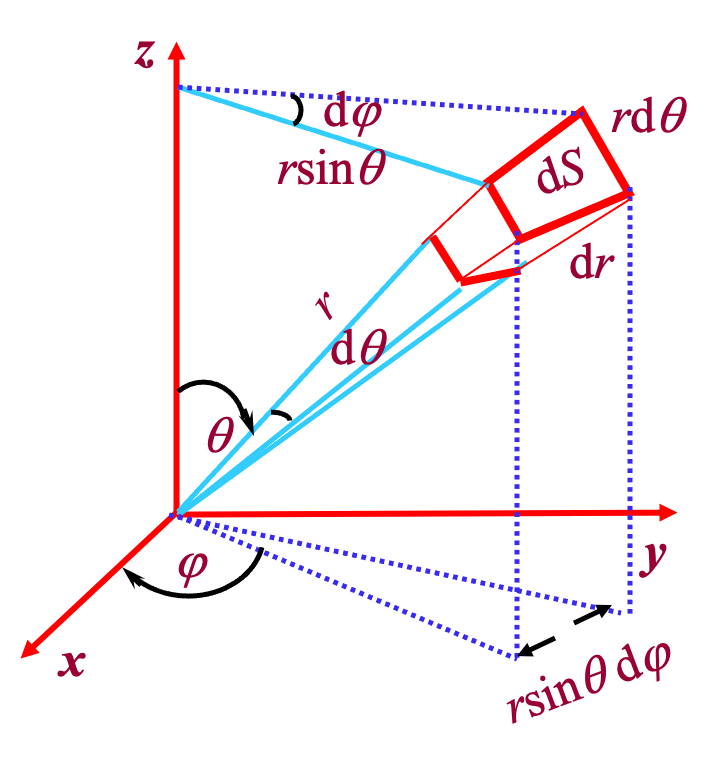
\includegraphics[width=0.4\textwidth]{figs/dt.png}
  \end{center}
$$ \begin{aligned}
  dS&=(rd\theta)\cdot (r\sin \theta d \varphi ) =r^2 \sin \theta d\theta d \varphi \\
  d \tau &=dS \cdot dr = r^2 \sin \theta dr d\theta d \varphi	  
\end{aligned}$$
\end{frame}

\begin{frame}
	* 求 $N_{nl}$ 
	\begin{equation*}
	\begin{split}
		\iiint  &\Psi(r,\theta,\varphi) d \tau =1  \\
		\iiint  &|N_{nl} R (r) Y_{lm} (\theta,\varphi)| ^2 r^2 \sin \theta dr d\theta d\varphi =1  \\
		\int_{0}^{\infty}  & N^2_{nl} R^2  (r)  r^2 dr =1   \\
		\frac{1}{\alpha ^3}	&\int_{0}^{\infty}  N^2_{nl}  R^2 (\xi)  \xi^2 d\xi =1   \\
		\frac{1}{\alpha ^3} &	\int_{0}^{\infty}  N^2_{nl}  \xi ^{2l+2}  [L_{n-l-1} ^{2l+1} (\xi)]^2 e^{-\xi}  d\xi =1   \\
		\frac{1}{\alpha ^3} &	\int_{0}^{\infty}  N^2_{nl}  \xi ^{M+1}  [L_N ^M (\xi)]^2 e^{-\xi}  d\xi =1   \\
	\end{split}		
	\end{equation*}	
\end{frame}		

\begin{frame}
	\begin{equation*}
		\frac{1}{\alpha ^3} 	  N^2_{nl}  \frac{(N+M)!}{N!} (2N+M+1) =1  	
	\end{equation*}	
	$\to$ \\
	\begin{equation*}
		N^2 _{nl}  \frac{2n [(n+1)!]^3} {\alpha^3 (n-l-1)!} =1
	\end{equation*}	
	\begin{equation*}
		N_{nl}  =\sqrt{\alpha^3 \frac{ (n-l-1)!}{2n [(n+1)!]^3}} 
	\end{equation*}	
\end{frame}		

\section{5.氢原子量子描述}

\begin{frame}
	\frametitle{小结:解氢原子}
	\tcbset{enhanced jigsaw,fonttitle=\bfseries,opacityback=0.35,colback=blue!5!white,
		frame style={left color=red!75!black,right color=red!10!yellow}}
	
\begin{tikzpicture}% draw two balls
	  \path[use as bounding box] (0,0.8) rectangle +(0.1,0.1);
	  \shadedraw [shading=ball] (0,0.3) circle (1cm);
	  %\shadedraw [ball color=yellow!20] (3,-2.2) circle (1cm);
	\end{tikzpicture}
	\begin{tcolorbox}[title=\faEnvira\hspace{1em} 第一次分离变量,
	  overlay=
	  {\begin{tcbinvclipframe}
	  \draw[red,line width=1cm] ([xshift=-2mm,yshift=2mm]frame.north west)
	  --([xshift=2mm,yshift=-2mm]frame.south east);
	  \draw[red,line width=1cm] ([xshift=-2mm,yshift=-2mm]frame.south west)
	  --([xshift=2mm,yshift=2mm]frame.north east);
	  \end{tcbinvclipframe}}]
	  {\Bullet}氢原子定态薛定谔方程:
		\begin{equation*}
			\left[-\frac{\hbar^2}{2 m_1} \nabla_1 ^2  -\frac{\hbar^2}{2 m_2} \nabla_2 ^2 +U(| \vec{r_1}-\vec{r_2} | ) \right] \Psi (\vec{r_1},\vec{r_2}) =E \Psi (\vec{r_1},\vec{r_2}) 
		\end{equation*}
	{\Bullet} 质心运动方程
	  \begin{equation*}
		-\frac{\hbar^2}{2 M} \nabla_R ^2  \psi (\vec{R}) =E_c \psi (\vec{R}) 
	\end{equation*}	
	{\Bullet} 相对运动方程
	\begin{equation*}
		\left[-\frac{\hbar^2}{2 m} \nabla ^2 +U(\vec{r}) \right] \Psi (\vec{r}) =E \Psi (\vec{r})   
	\end{equation*}
	  \end{tcolorbox}
\end{frame}

\begin{frame}
	\frametitle{}
	\tcbset{enhanced jigsaw,fonttitle=\bfseries,opacityback=0.35,colback=blue!5!white,
		frame style={left color=red!75!black,right color=red!10!yellow}}
	
\begin{tikzpicture}% draw two balls
	  \path[use as bounding box] (0,0.8) rectangle +(0.1,0.1);
	  \shadedraw [shading=ball] (0,0.3) circle (1cm);
	  %\shadedraw [ball color=yellow!20] (3,-2.2) circle (1cm);
	\end{tikzpicture}
	\begin{tcolorbox}[title=\faEnvira\hspace{1em} 第二次分离变量,
	  overlay=
	  {\begin{tcbinvclipframe}
	  \draw[red,line width=1cm] ([xshift=-2mm,yshift=2mm]frame.north west)
	  --([xshift=2mm,yshift=-2mm]frame.south east);
	  \draw[red,line width=1cm] ([xshift=-2mm,yshift=-2mm]frame.south west)
	  --([xshift=2mm,yshift=2mm]frame.north east);
	  \end{tcbinvclipframe}}]
	{\Bullet}角向方程:
	\begin{equation*}
		\left[ \frac{1}{ \sin \theta  } \frac{\partial }{\partial \theta } (\sin \theta \frac{\partial }{\partial \theta } )
		+\frac{1}{ \sin^2 \theta  } \frac{\partial^2}{\partial\varphi ^2}  +l(l+1) \right] Y=0 
	\end{equation*}
	{\Bullet}径向方程:
	\begin{equation*}
		\frac{d^2 R}{d r^2} + \frac{2}{r^2}\frac{d R }{d r}  + \frac{2 \mu} {\hbar^2}(E+ \frac{e_s ^2}{r} ) R- \frac{l(l+1)}{r^2} R=0
	\end{equation*}	
	  \end{tcolorbox}
\end{frame}

\begin{frame}
	\frametitle{}
	\tcbset{enhanced jigsaw,fonttitle=\bfseries,opacityback=0.35,colback=blue!5!white,
		frame style={left color=red!75!black,right color=red!10!yellow}}
	
\begin{tikzpicture}% draw two balls
	  \path[use as bounding box] (0,0.8) rectangle +(0.1,0.1);
	  \shadedraw [shading=ball] (0,0.3) circle (1cm);
	  %\shadedraw [ball color=yellow!20] (3,-2.2) circle (1cm);
	\end{tikzpicture}
	\begin{tcolorbox}[title=\faEnvira\hspace{1em} 第三次分离变量,
	  overlay=
	  {\begin{tcbinvclipframe}
	  \draw[red,line width=1cm] ([xshift=-2mm,yshift=2mm]frame.north west)
	  --([xshift=2mm,yshift=-2mm]frame.south east);
	  \draw[red,line width=1cm] ([xshift=-2mm,yshift=-2mm]frame.south west)
	  --([xshift=2mm,yshift=2mm]frame.north east);
	  \end{tcbinvclipframe}}]
	{\Bullet}经度方程:
	\begin{equation*}
		\frac{d^{2} \Phi}{d \varphi^{2}}+\lambda \Phi=0,(0<\varphi\le2 \pi)
	\end{equation*}	
	{\Bullet}纬度方程:
	\begin{equation*}
		\frac{1}{\sin \theta} \frac{d}{d \theta}\left(\sin \theta \frac{d \Theta}{d \theta}\right)+\left[l(l+1)-\frac{\lambda}{\sin ^{2} \theta}\right] \Theta=0,(0<\theta \le \pi)
	\end{equation*}	
	{\Bullet}径向方程:
	\begin{equation*}
		\frac{d^2 R}{d r^2} + \frac{2}{r^2}\frac{d R }{d r}  + \frac{2 \mu} {\hbar^2}(E+ \frac{e_s ^2}{r} ) R- \frac{l(l+1)}{r^2} R=0
	\end{equation*}	
	  \end{tcolorbox}
\end{frame}

\begin{frame}
	\frametitle{}
	\tcbset{enhanced jigsaw,fonttitle=\bfseries,opacityback=0.35,colback=blue!5!white,
		frame style={left color=red!75!black,right color=red!10!yellow}}
	
\begin{tikzpicture}% draw two balls
	  \path[use as bounding box] (0,0.8) rectangle +(0.1,0.1);
	  \shadedraw [shading=ball] (0,0.3) circle (1cm);
	  %\shadedraw [ball color=yellow!20] (3,-2.2) circle (1cm);
	\end{tikzpicture}
	\begin{tcolorbox}[title=\faEnvira\hspace{1em} 经度方程的解,
	  overlay=
	  {\begin{tcbinvclipframe}
	  \draw[red,line width=1cm] ([xshift=-2mm,yshift=2mm]frame.north west)
	  --([xshift=2mm,yshift=-2mm]frame.south east);
	  \draw[red,line width=1cm] ([xshift=-2mm,yshift=-2mm]frame.south west)
	  --([xshift=2mm,yshift=2mm]frame.north east);
	  \end{tcbinvclipframe}}]
	{\Bullet}经度方程:
	\begin{equation*}
		\frac{d^{2} \Phi}{d \varphi^{2}}+\lambda \Phi=0,(0<\varphi\le2 \pi)
	\end{equation*}	
	固有值和固有函数:
	\[\begin{cases}
		\lambda=m^2, ~~~ (m=0,\pm 1,\pm 2,\cdots,\pm l) \\ 
		\Phi_m (\varphi)=\frac{1}{\sqrt{2\pi}} e^{im\varphi}
	\end{cases}\]
	物理上对应角动量Z方向投影:
	\[L_z =m\hbar \]
	\end{tcolorbox}
\end{frame}

\begin{frame}
	\frametitle{}
	\tcbset{enhanced jigsaw,fonttitle=\bfseries,opacityback=0.35,colback=blue!5!white,
		frame style={left color=red!75!black,right color=red!10!yellow}}
	
\begin{tikzpicture}% draw two balls
	  \path[use as bounding box] (0,0.8) rectangle +(0.1,0.1);
	  \shadedraw [shading=ball] (0,0.3) circle (1cm);
	  %\shadedraw [ball color=yellow!20] (3,-2.2) circle (1cm);
	\end{tikzpicture}
	\begin{tcolorbox}[title=\faEnvira\hspace{1em} 纬度方程的解,
	  overlay=
	  {\begin{tcbinvclipframe}
	  \draw[red,line width=1cm] ([xshift=-2mm,yshift=2mm]frame.north west)
	  --([xshift=2mm,yshift=-2mm]frame.south east);
	  \draw[red,line width=1cm] ([xshift=-2mm,yshift=-2mm]frame.south west)
	  --([xshift=2mm,yshift=2mm]frame.north east);
	  \end{tcbinvclipframe}}]
	  {\Bullet}纬度方程:
	  \begin{equation*}
		  \frac{1}{\sin \theta} \frac{d}{d \theta}\left(\sin \theta \frac{d \Theta}{d \theta}\right)+\left[l(l+1)-\frac{m^2}{\sin ^{2} \theta}\right] \Theta=0,(0<\theta \le \pi)
	  \end{equation*}	
	固有值
	\[\begin{cases}
		 m^2, ~~~ (m=0,\pm 1,\pm 2,\cdots,\pm l) \\
		l(l+1), ~~~ (l=1, 2,\cdots, n-1) \\ 
	\end{cases}\]
	固有函数:
	\[
		\Theta_{lm}(\theta)= P^m  _{l}(\cos \theta) \]
\end{tcolorbox}
\end{frame}

\begin{frame}
	\frametitle{}
	\tcbset{enhanced jigsaw,fonttitle=\bfseries,opacityback=0.35,colback=blue!5!white,
		frame style={left color=red!75!black,right color=red!10!yellow}}
	
\begin{tikzpicture}% draw two balls
	  \path[use as bounding box] (0,0.8) rectangle +(0.1,0.1);
	  \shadedraw [shading=ball] (0,0.3) circle (1cm);
	  %\shadedraw [ball color=yellow!20] (3,-2.2) circle (1cm);
	\end{tikzpicture}
	\begin{tcolorbox}[title=\faEnvira\hspace{1em} 角向方程的解,
	  overlay=
	  {\begin{tcbinvclipframe}
	  \draw[red,line width=1cm] ([xshift=-2mm,yshift=2mm]frame.north west)
	  --([xshift=2mm,yshift=-2mm]frame.south east);
	  \draw[red,line width=1cm] ([xshift=-2mm,yshift=-2mm]frame.south west)
	  --([xshift=2mm,yshift=2mm]frame.north east);
	  \end{tcbinvclipframe}}]
	{\Bullet}角向方程:
	\begin{equation*}
		\left[ \frac{1}{ \sin \theta  } \frac{\partial }{\partial \theta } (\sin \theta \frac{\partial }{\partial \theta } )
		+\frac{1}{ \sin^2 \theta  } \frac{\partial^2}{\partial\varphi ^2}  +l(l+1) \right] Y=0 
	\end{equation*}
	角动量固有值
	\[\begin{cases}
		m\hbar, ~~~ (m=0,\pm 1,\pm 2,\cdots,\pm l) \\
		l(l+1)\hbar^2, ~~~ (l=1, 2,\cdots, n-1) \\ 
	\end{cases}\]
	固有函数:
	\[
		Y_{lm} (\theta,\varphi)= \sqrt{\frac{(2l+1)(l-m)!}{4\pi (l+m)!}}  P_l ^m (cos \theta)  e^{im\varphi}  \]
\end{tcolorbox}
\end{frame}

\begin{frame}
	\frametitle{}
	\tcbset{enhanced jigsaw,fonttitle=\bfseries,opacityback=0.35,colback=blue!5!white,
		frame style={left color=red!75!black,right color=red!10!yellow}}
	
\begin{tikzpicture}% draw two balls
	  \path[use as bounding box] (0,0.8) rectangle +(0.1,0.1);
	  \shadedraw [shading=ball] (0,0.3) circle (1cm);
	  %\shadedraw [ball color=yellow!20] (3,-2.2) circle (1cm);
	\end{tikzpicture}
	\begin{tcolorbox}[title=\faEnvira\hspace{1em} 径向方程的解,
	  overlay=
	  {\begin{tcbinvclipframe}
	  \draw[red,line width=1cm] ([xshift=-2mm,yshift=2mm]frame.north west)
	  --([xshift=2mm,yshift=-2mm]frame.south east);
	  \draw[red,line width=1cm] ([xshift=-2mm,yshift=-2mm]frame.south west)
	  --([xshift=2mm,yshift=2mm]frame.north east);
	  \end{tcbinvclipframe}}]
	  {\Bullet}径向方程:
	  \begin{equation*}
		\frac{d^2 R}{d r^2} + \frac{2}{r^2}\frac{d R }{d r}  + \frac{2 \mu} {\hbar^2}(E+ \frac{e_s ^2}{r} ) R- \frac{l(l+1)}{r^2} R=0
	  \end{equation*}	
	能量固有值
	\[ E_n =- \frac{1}{n^2} \frac{\mu e^4 _s }{2 \hbar ^2} =\frac{E_1}{n^2}, \qquad (n=1,2,3,\cdots) \]
	固有函数:
	\[
		R_{nl} (r) =\sqrt{(\frac{2}{n a_0})^3 \frac{ (n-l-1)!}{2n [(n+1)!]^3}}  (\frac{2}{n a_0}r) ^l  L_{n-l-1} ^{2l+1} (\frac{2}{n a_0}r) e^{-\frac{r}{n a_0}}\]
\end{tcolorbox}
\end{frame}


\begin{frame}
	\frametitle{}
	\tcbset{enhanced jigsaw,fonttitle=\bfseries,opacityback=0.35,colback=blue!5!white,
		frame style={left color=red!75!black,right color=red!10!yellow}}
	
\begin{tikzpicture}% draw two balls
	  \path[use as bounding box] (0,0.8) rectangle +(0.1,0.1);
	  \shadedraw [shading=ball] (0,0.3) circle (1cm);
	  %\shadedraw [ball color=yellow!20] (3,-2.2) circle (1cm);
	\end{tikzpicture}
	\begin{tcolorbox}[title=\faEnvira\hspace{1em} 氢原子的解,
	  overlay=
	  {\begin{tcbinvclipframe}
	  \draw[red,line width=1cm] ([xshift=-2mm,yshift=2mm]frame.north west)
	  --([xshift=2mm,yshift=-2mm]frame.south east);
	  \draw[red,line width=1cm] ([xshift=-2mm,yshift=-2mm]frame.south west)
	  --([xshift=2mm,yshift=2mm]frame.north east);
	  \end{tcbinvclipframe}}]
	  {\Bullet}	氢原子波函数:
	\begin{equation*}	
		 \Psi_{nlmm_s}(r, \theta, \varphi, s)= R_{nl} (r) Y_{lm} (\theta,\varphi)S_{m_s}(s)
	\end{equation*} 
	\begin{itemize}
		  \item 主量子数: $n=1,2,3,\cdots$, 能级,轨道能量 (主 K,L,M, N, O, P, Q)
		  \item 角量子数: $l=0,1,2,\cdots, n-1$, 角动量大小, 轨道形状 (次 s, p, d, f) 
		  \item 磁量子数: $m=0,\pm 1,\pm 2,\cdots, \pm l$, 角动量方向, 轨道空间取向 
		  \item 自旋量子数: $m_s=\pm 1/2$
	\end{itemize}
\end{tcolorbox}
\end{frame}


\begin{frame}
	  \frametitle{轨道波函数}
	  \begin{center}
		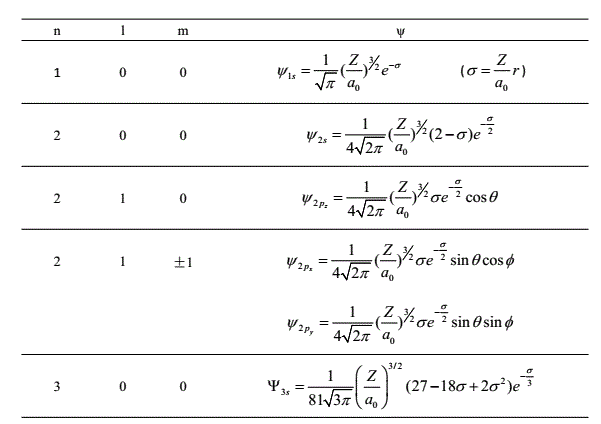
\includegraphics[width=0.95\textwidth]{figs/orbitals.png}
   \end{center}
\end{frame}

\begin{frame}
	  \frametitle{能级与光谱}
	  \[ E_n = - \frac{1}{n^2} \frac{\mu e^4 _s }{2 \hbar ^2} =\frac{E_1}{n^2}, \quad (n=1,2,3,\cdots) , \qquad \nu=\frac{E_n -E_m}{h} = R_H c [\frac{1}{m^2} -\frac{1}{n^2}]
	  \]
	  \begin{center}
		   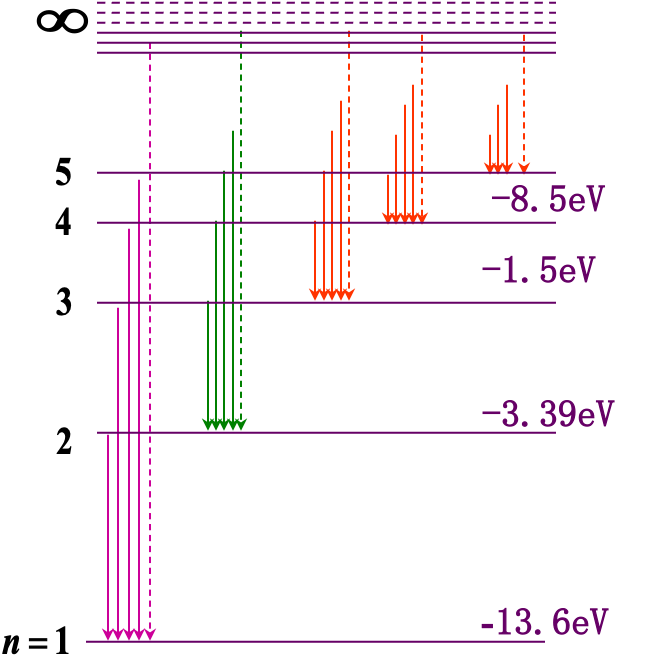
\includegraphics[width=0.40\textwidth]{figs/spectra.png}
	  \end{center}
\end{frame}

\begin{frame} 
    \frametitle{角动量量子化}
    \begin{wrapfigure} {b} {0.4\textwidth} %;图在右
        \includegraphics[width=0.35\textwidth]{figs/LandL2.png}   
    \end{wrapfigure}
    {\Bullet} 角动量大小  $L^2=l(l+1) \hbar^2$\\
	$L=\sqrt{l(l+1)}\hbar, \quad (l=1,2,\cdots, n-1)$\\
    ~~\\ \vspace{0.3em}
    {\Bullet} 角动量Z投影 $L^2_z=m^2\hbar^2$\\
    $L_z=m\hbar, \quad (m=0,\pm 1,\pm 2, \cdots, \pm l)$\\
	~~\\
    {\Bullet} 大小和方向皆量子化
\end{frame} 

\begin{frame}
	  \frametitle{轨道的形态}
		\begin{center}
			 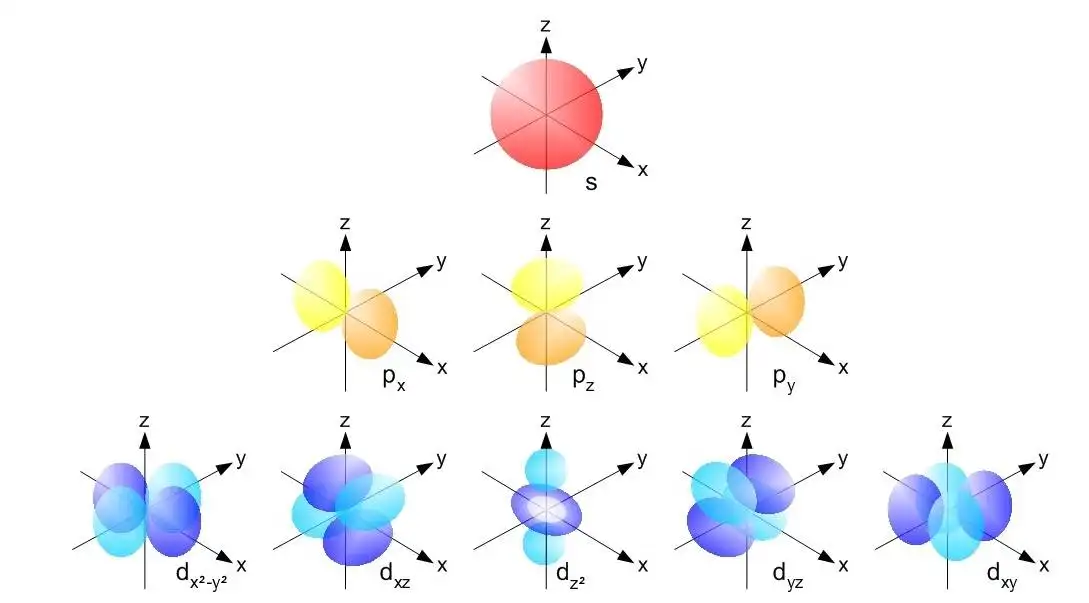
\includegraphics[width=1.0\textwidth,height=2.5in]{figs/2022-03-25-19-35-50.png}
		\end{center}	 
\end{frame}	

\begin{frame}
	  \frametitle{}
	  \例 [求电子云的形态]{}
	  \begin{enumerate}
		  \item 径向分布($r-r+dr$找到粒子的概率)
		   \[ \begin{aligned}
	    \omega_{nl} dr &= \int _{\varphi=0} ^{2\pi} \int _{\theta=0} ^{\pi} |R_{nl}(r)Y_{lm}(\theta,\varphi)|^2 r^2\sin \theta dr d\theta d \varphi \\
		&= R^2_{nl}(r) r^2 dr \\
		\end{aligned}\]
		\item 角向分布($(\theta,\varphi)-(\theta+d\theta,\varphi+d\varphi)$找到粒子的概率)		
		\[ \begin{aligned}
			\omega_{lm} d \Omega &= \int _{r=0} ^{\infty} |R_{nl}(r)Y_{lm}(\theta,\varphi)|^2 r^2dr  d \Omega \\
			&= |Y_{lm}|^2 d \Omega 	
			\end{aligned}\]		
	  \end{enumerate}  
\end{frame}
%%%%%%%%%%%%%%%%%%%%%%%%%%%%%%%%%%%%%%%%%%%%%%
\begin{frame}
	\frametitle{}
  \begin{center}
	   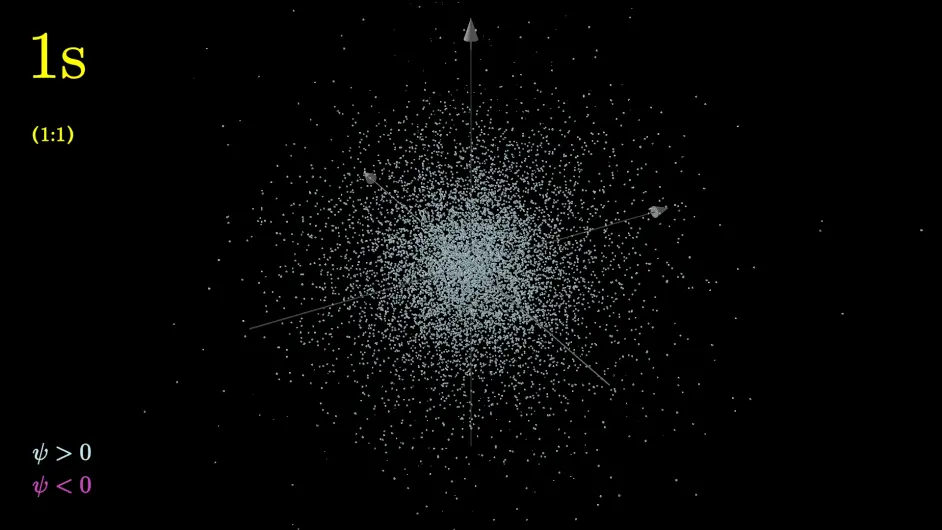
\includegraphics[width=1\textwidth]{figs/2022-03-30-18-45-45.png}
  \end{center}
\end{frame}

\begin{frame}
	\frametitle{}
  \begin{center}
	   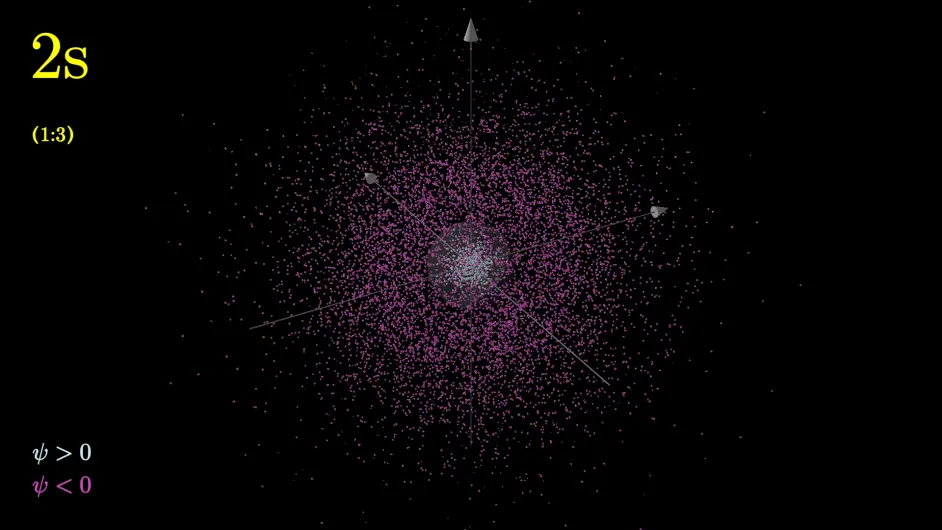
\includegraphics[width=1\textwidth]{figs/2022-03-30-18-46-37.png}
  \end{center}
\end{frame}

\begin{frame}
	\frametitle{}
  \begin{center}
	   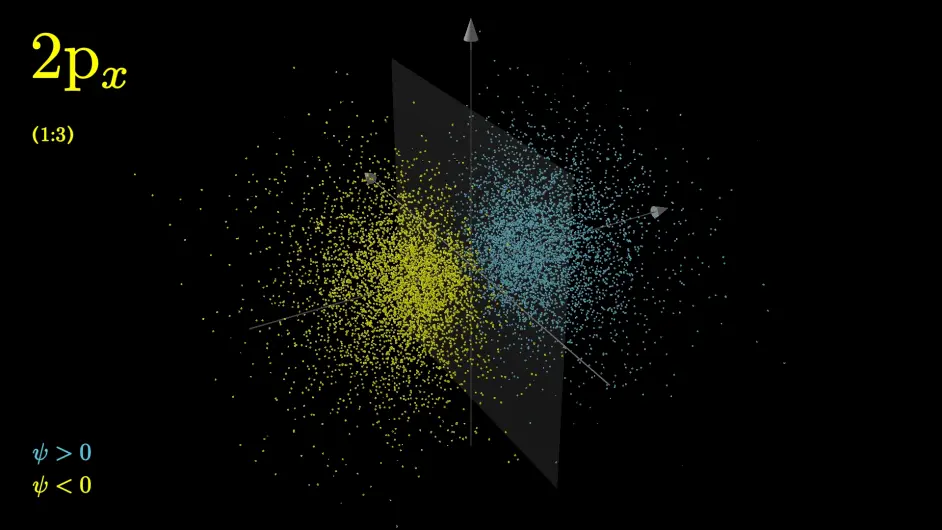
\includegraphics[width=1\textwidth]{figs/2022-03-30-18-48-34.png}
  \end{center}
\end{frame}

\begin{frame}
	\frametitle{}
  \begin{center}
	   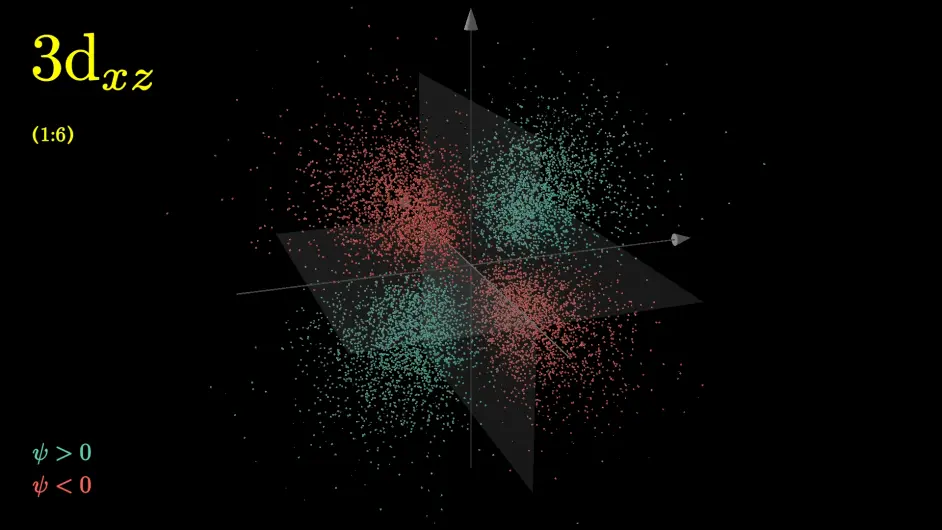
\includegraphics[width=1\textwidth]{figs/2022-03-30-18-49-45.png}
  \end{center}
\end{frame}

\begin{frame}
	\frametitle{}
  \begin{center}
	   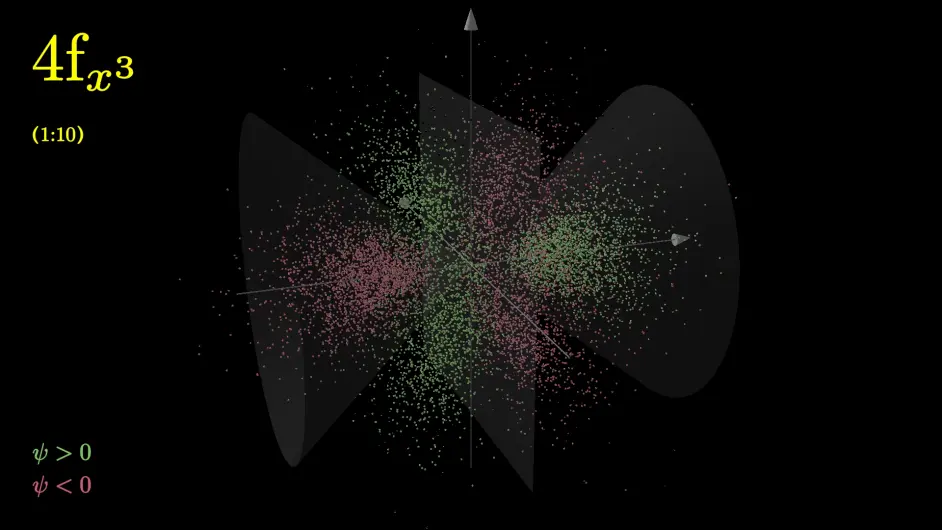
\includegraphics[width=1\textwidth]{figs/2022-03-30-18-55-10.png}
  \end{center}
\end{frame}

\begin{frame}
	\frametitle{作业}
	1、证明拉盖多项式的正交性\\
	2、求方程的解
	\begin{equation*}
		\frac{d^2 U}{d \xi ^2} + \frac{2}{\xi }\frac{d U }{d \xi}  +[\frac{\beta}{\xi} - \frac{l(l+1)}{\xi ^2}] U=0
	\end{equation*}	 
	3、计算积分:
	\begin{equation*}
		\int_{0}^{\infty}   e^{-x} ( L_1 (x) )^2 dx, \qquad  \int_{0}^{\infty}   e^{-x} ( L_2 (x) )^2 dx, 
	\end{equation*}	
	4、写出 $L_1 (x)$ 和 $L_1 ^0 (x)$ 之间的关系式
\end{frame}		

\begin{frame}
	\frametitle{随堂测试}
	\begin{exampleblock} {1.粒子处于如下势场中:}
		\begin{equation*}
			V(x)= \frac{1}{2} \mu \omega ^2 x^2  +1
		\end{equation*}
		\hspace{2em}求能量固有值和定态波函数。
	\end{exampleblock}	
	\begin{exampleblock} {2.基于厄米多项式的正交性求积分:}
		\begin{equation*}
			\int\limits_{-\infty}^{+\infty} (x^3 +1)e^{-x^{2}} H_n(x) d x 
		\end{equation*}
	\end{exampleblock}	
\end{frame}


\begin{frame}
	\frametitle{}
	\begin{exampleblock} {1.粒子处于如下势场中:}
	  \begin{equation*}
		  V(x)= \frac{1}{2} \mu \omega ^2 x^2  +1
	  \end{equation*}
	\end{exampleblock}
	  \hspace{2em}求能量固有值和定态波函数。\\	
	  \解 ~ (1)含时分离变量, 得时间函数: $T(t)  = \exp(-i E t /\hbar) $ \\
	  (2) 定态薛定谔方程:
	  \begin{equation*}
		  \begin{split}
			  \left [ -\frac{\hbar^2}{2\mu} \frac{\mathrm{d} ^2}{\mathrm{d} x^2} +\frac{1}{2}\mu \omega^2 x^2 +1 \right ]\Psi(x)&=E\Psi(x) \\ 
			  \left [ -\frac{\hbar^2}{2\mu} \frac{\mathrm{d} ^2}{\mathrm{d} x^2} +\frac{1}{2}\mu \omega^2 x^2  \right ]\Psi(x)&=(E-1)\Psi(x) 	
		  \end{split}
	  \end{equation*}
	  令 $E'=E-1$, 得:
	  \[\left [ -\frac{\hbar^2}{2\mu} \frac{\mathrm{d} ^2}{\mathrm{d} x^2} +\frac{1}{2}\mu \omega^2 x^2  \right ]\Psi(x)=E'\Psi(x) \]
	  此方程就是谐振子标准方程!
\end{frame}

\begin{frame}
		\frametitle{}	  
	  能量固有值(能级$E_n$)
	  \begin{equation*}
		  E'_n=\left(n+\frac{1}{2}\right) \hbar \omega=E_n-1, ~~~  ( n=0,1,2, ...)  
	  \end{equation*}  
	  定态波函数为
	  \begin{equation*}
		  \Psi_n(x,t) = \left( \frac{\alpha}{\sqrt{\pi} 2^n n!}  \right) ^{1/2}  \exp(-\frac{ \alpha^2 x^2}{2} -\frac{i}{\hbar} E_n t ) H( \alpha x) , \qquad (\alpha ^2= \frac{\mu\omega}{\hbar}) 
	  \end{equation*}  
\end{frame}